\documentclass[11pt,a4paper]{article}

\usepackage[utf8]{inputenc}
\usepackage[T1]{fontenc}
\usepackage{lmodern}
\usepackage[margin=1in]{geometry}
\usepackage{setspace}
\usepackage{amsmath,amssymb}
\usepackage{booktabs}
\usepackage{graphicx}
\usepackage{natbib}
\usepackage{authblk}
\usepackage{xcolor}
\usepackage{tikz}
\usepackage{float}
\usepackage{array}
\usepackage{hyperref}

\doublespacing
\setlength{\parskip}{0.3em}
\setlength{\emergencystretch}{2em}
\clubpenalty=10000
\widowpenalty=10000
\displaywidowpenalty=10000
\setcitestyle{aysep={}}
\hypersetup{
  colorlinks=true,
  linkcolor=blue!45!black,
  citecolor=blue!45!black,
  urlcolor=blue!45!black
}

\title{AI, Fiscal Space, and Social Protection in Four Latin American Economies:\\[0.2em]
A Scenario-Based Threshold Framework}
\author{Vicenzo Scavino\thanks{Corresponding author. Email: \href{mailto:vicenzoscavino52@gmail.com}{vicenzoscavino52@gmail.com}. ORCID: \href{https://orcid.org/0009-0000-2472-9785}{0009-0000-2472-9785}.}}
\affil{Independent Researcher, Lima, Peru}
\date{}

\begin{document}

\maketitle

\begin{center}\small Running title: AI, Fiscal Space, and Social Protection\end{center}

\begin{abstract}
Can fiscal space generated by artificial intelligence finance recurrent social protection in Latin America? This paper develops a scenario-based fiscal-feasibility test that translates an AI dividend into domestic income and fiscal capture, compares it with policy costs on a common denominator, and adds debt-consistency and persistence screens. Applied to Peru, Chile, Colombia, and Mexico, its primary channel-based specification yields no deterministic crossing in the non-stress scenarios (low, mid, frontier): domestic translation and fiscal capture jointly fall short. Crossings arise only in a diagnostic disruptive scenario. Chilean guaranteed minimum income is conditionally feasible and debt-consistent; Peru's social pension crosses the accounting threshold but fails the debt guardrail; Colombia and Mexico do not cross. Crossing frequencies are model-implied across calibrated draws, not predictive probabilities. The primary specification was fixed in advance, and the persistence horizon is a derived post-baseline extension. The framework identifies when an AI dividend could sustain a recurrent commitment.
\end{abstract}

\noindent \textbf{Keywords:} artificial intelligence, fiscal space, universal social protection, universal basic income, informality, fiscal capacity, labor share, emerging economies, Latin America.\\
\textbf{JEL codes:} O33, H53, H24, I38, O54, E62.

\newpage

\section{Introduction}\label{sec:introduction}

Can fiscal space generated by artificial intelligence finance recurrent social protection in Latin American economies---and, if so, when? AI may raise output, alter factor incomes, and expand taxable bases. Social pensions, minimum-income guarantees, and universal transfers, however, create commitments that must be financed repeatedly rather than at a favorable point in time. The relevant policy question is therefore not whether an AI dividend is conceivable. It is whether, under explicit scenarios and for long enough, that dividend can be translated into domestic income, captured by the public sector, and made available after policy costs and debt requirements are recognized. That timing distinction matters for budget design: a large eventual dividend cannot support a current entitlement unless its fiscal transmission and duration are credible. Answering the question comparably across countries and instruments requires a common financing test rather than a forecast attached to a single program.

Each link in that chain is uncertain. Macroeconomic gains depend on which tasks AI affects and how those gains diffuse, while automation can change the distribution of income across tax bases \citep{acemoglu2024simple,acemoglu2019automation}. Fiscal policy can broaden or narrow the distribution of AI gains, but effective capture depends on the existing tax architecture, behavioral responses, and administrative capacity \citep{brollo2024fiscal,korinek2026public,gaspar2016tax}. Exposure is therefore not adoption; additional output is not automatically taxable income; and additional revenue is not necessarily debt-consistent fiscal space. These distinctions motivate a threshold exercise that keeps the technological, domestic, fiscal, and policy-cost objects separate.

Two strands of work come closest to the question. AI--universal-basic-income (UBI) models study particular financing arrangements: \citet{nayebi2025threshold} derives an AI-capability threshold for rent-funded UBI in the United States, while \citet{ito2026ubi} simulates UBI feasibility for Japan with dynamic social-security offsets. They move beyond pure incidence, but retain one country and one instrument. In the policy-modeling tradition, \citet{caamal2022ubi} evaluate UBI in Mexico and \citet{lara2026basic} study a basic-income--flat-tax reform in Spain through country-specific tax-benefit simulations. Those studies identify poverty, inequality, efficiency, or budget effects at a specified policy configuration. None provides the comparative dynamic-fiscal test posed here: when, and in which country--instrument--scenario cells, can a projected AI dividend sustain a recurrent commitment after domestic translation and fiscal capture, on a common denominator, while satisfying debt consistency and a required duration? This paper contributes that test. It complements static incidence analysis rather than replacing it: the object is not how much a transfer redistributes at one point in time, but under which conditions its projected financing source can persist.

The framework implements this comparison as a modular chain. An external AI scenario is first translated into domestic income. The income increment is allocated across labor and nonlabor bases and converted into effective fiscal space through marginal fiscal conversion (MFC). That flow is compared with the harmonized cost of each instrument through the feasibility ratio $V$, with the accounting crossing defined by $V\geq1$. A separate guardrail asks whether the same flow can finance the instrument while meeting the primary-balance correction implied by the maintained debt path. Diagnostic inversions then recover the gain, fiscal conversion, and domestic translation required to reach the boundary. A final inversion, $H^*$, reports the required persistence horizon; it is a derived post-baseline extension, not a forecast date, and changes no calibrated input or baseline classification.

The application covers four economies selected for contrast rather than regional representativeness: Peru, Chile, Colombia, and Mexico. They differ in policy costs, fiscal architectures, and debt space. The instrument set spans categorical, targeted, and broad universal commitments, all priced on the same endpoint-GDP denominator. A common scenario grid changes the technological input, while the fiscal regimes change effective capture without relabeling that input. This separation gives a crossing the same accounting meaning across country--instrument cells and shows whether debt consistency changes the classification. The purpose is not to rank the welfare value of the programs, but to test the sufficiency of a specified financing source under transparent and comparable conditions.

The first result is a deterministic non-crossing under the primary channel-based specification across the non-stress scenarios (low, mid, and frontier). The largest accounting ratio is only $V=0.177$. The gap is joint: domestic translation at the maintained fiscal architecture is insufficient, but reform-level capture at the maintained technological gain is also insufficient. At the maintained prudential buffer, every mid-scenario translation inversion requires $T^{req,H}>1$, and the lowest AI-rent capture requirement is 13.50 times the strongest specified upper support. The evidence therefore supports neither ``translation, not taxation'' nor its inverse. Translation and capture are complementary links, and neither closes the non-stress gap alone. In the primary Monte Carlo, the largest non-stress crossing frequency is 2.36 percent. This is a model-implied frequency across calibrated draws, conditional on stated supports and distributional assumptions, not a predictive probability of real-world financing.

Deterministic crossings appear only under the disruptive scenario, which is a diagnostic stress test rather than a central projection. Chile's guaranteed minimum income (GMI) is the sole conditionally feasible country--instrument result: it crosses in both the ideal and targeting-cost-loaded variants and passes the debt guardrail. Peru's social pension crosses the accounting boundary under stress but fails debt consistency, making it the fragile case rather than a fiscal green light. Colombia and Mexico do not cross in any evaluated cell. These negative findings are informative because every cell faces the same financing condition; they delimit what the stated scenarios can support instead of leaving non-feasibility unmeasured. The persistence extension reinforces the conditional reading by asking how long a shock must endure, not when adoption will occur. The ICT placebo, reduced-form exposure-rescaling diagnostic, channel ablations, and source-substitution exercise further test whether the crossing pattern is specific to the maintained channels.

The policy contribution is consequently narrow but operational. Prospective AI revenues should not be booked as short-run financing for universal social protection, and fiscal reform cannot be treated as a substitute for realizing the domestic productive gain. The threshold framework instead identifies the evidence that would warrant reassessment: realized translation, effective capture, debt consistency, and sufficient persistence. After the next section positions the paper in the literature, Sections~\ref{sec:framework} and~\ref{sec:design} develop and operationalize the test. Section~\ref{sec:results} presents the evidence, and Sections~\ref{sec:discussion} and~\ref{sec:conclusion} draw out its policy implications and conclude.

\section{Related Literature and Contribution}\label{sec:literature}

The financing question posed in Section~\ref{sec:introduction} draws on five strands of research, each addressing a different link between a technological gain and a recurrent social commitment. The relevant distinction is between what each strand disciplines and what it leaves unresolved. Read in sequence, the literatures identify the uncertainty in the aggregate shock, its allocation across factor incomes, its conversion into public revenue, and the cost of the policy to be financed.

\paragraph{Macroeconomic effects of AI and automation.}
Macroeconomic assessments span task accounting, micro-to-macro aggregation, and evidence on technology diffusion. Syntheses that organize AI's productivity, distributional, and growth channels do not collapse them into a single aggregate path \citep{oecd2024impactai}. Task-based models begin with the activities that technology can perform and aggregate from their economic weight, the associated cost savings, and the creation or reinstatement of tasks \citep{acemoglu2018race,acemoglu2019automation,acemoglu2024simple}. This approach makes occupational exposure an input rather than an aggregate growth estimate. A complementary micro-to-macro literature combines task-level performance, exposure, adoption, and propagation across sectors to construct aggregate productivity paths, including frontier applications under high exposure and adoption \citep{filippucci2024miracle,oecd2025g7}. Field and experimental studies document productivity gains in particular work settings and professional writing tasks \citep{brynjolfsson2023generative,noy2023experimental}. Cross-country evidence on earlier technologies documents substantial heterogeneity in adoption timing across technologies and economies \citep{comin2010diffusion}. Complementary intangible investment can also delay the appearance of gains in measured productivity, producing a productivity J-curve rather than immediate realization \citep{brynjolfsson2021jcurve}. Preparedness-based analysis therefore treats digital infrastructure, skills, innovation linkages, and institutions as conditions for converting exposure into use \citep{cazzaniga2024genai}. These studies discipline task-level gains, diffusion, and timing, but do not by themselves identify aggregate output or the tax bases produced by diffusion. The aggregation exercises, in turn, depend on assumptions about adoption and transmission beyond the settings in which performance is observed \citep{acemoglu2024simple,filippucci2024miracle}. This strand therefore narrows plausible mechanisms without selecting a single magnitude, diffusion speed, or duration for the aggregate shock. Those open margins motivate a scenario input rather than a point forecast.

\paragraph{Distributional incidence and factor allocation.}
Automation can change both output and its allocation. In the task framework, displacement transfers activities away from labor, while reinstatement creates new labor-intensive tasks; productivity and labor income therefore need not move proportionately \citep{acemoglu2018race,acemoglu2019automation}. Regional labor-market mapping distinguishes exposure associated with productivity-enhancing transformation from automation risk and identifies the digital divide as a constraint on realizing the former \citep{worldbankilo2024lacgenai}. The wider factor-share literature likewise treats the division between labor and nonlabor income as an empirical object rather than a fixed accounting constant \citep{karabarbounis2014global}. Measurement adds a second distinction. Labor income must be adjusted for self-employment and mixed income, so the national-accounts residual outside measured employee compensation is not synonymous with corporate profit \citep{gollin2002getting}. It may contain mixed income, depreciation, operating surplus, and rents with different legal and fiscal treatments. An aggregate AI gain consequently does not reveal how much enters wages, taxable business income, consumption, or a separately reachable rent base. This literature establishes why factor allocation matters, but leaves the allocation of a particular projected increment across taxable bases unresolved.

\paragraph{Fiscal capacity and effective capture.}
Research on AI and public finance describes fiscal policy as a channel through which technological gains can be distributed and captured, using social protection, labor-market policy, and labor, capital, or corporate taxation \citep{brollo2024fiscal,korinek2026public}. Optimal-tax analyses of automation further show that the treatment of capital that substitutes for labor depends on the transition being considered and on the available tax instruments \citep{guerreiro2022robots}. Whether a proposed instrument produces revenue also depends on state capacity. \citet{besley2014taxation} relate tax collection in developing countries to investments in fiscal institutions, while \citet{jensen2022employment} links the expansion of employee taxation to the information generated by formal employment and third-party reporting. Work on tax capacity similarly distinguishes the reach of a tax system from the size of the underlying economy \citep{gaspar2016tax}. Panel estimates of tax buoyancy show that short- and long-run revenue responses differ by tax category and country group, so aggregate income growth need not map one-for-one into receipts \citep{dudine2018buoyancy}. That evidence disciplines historical capture comparisons, but does not identify the marginal response to an AI increment. These mechanisms create a wedge between economic income, a statutory rate, and realized marginal revenue. Behavioral base erosion, enforcement, and cross-border profit shifting belong in that mapping when corporate income is part of the base; reviews of international corporate tax avoidance document both multiple shifting channels and measurement blind spots \citep{beer2020international,brollo2024fiscal}. Nor is additional revenue alone a complete measure of fiscal space. Standard debt dynamics link the debt path to primary balances and growth-interest conditions, so a revenue-cost crossing does not establish debt consistency by itself \citep{escolano2010debt,imf2016fiscalspace}. The open object is thus effective, debt-consistent capture from a specified income increment, not the tax rate in isolation.

\paragraph{Social-protection design in economies with large informal sectors.}
Universal basic income, guaranteed minimum income, social pensions, and targeted transfers impose different eligibility, information, and budget requirements. Reviews of UBI therefore treat it as a policy architecture with explicit financing and interaction with existing benefits, rather than as a generic response to technological change \citep{gentilini2020ubi,oecd2017basicincome}. In developing-country settings, the comparison between universal and targeted transfers turns partly on imperfect information: proxy-means tests reduce coverage but introduce targeting errors when income is difficult to observe \citep{hanna2018universal}. Informal and non-employee work also limits the information available to tax and transfer systems \citep{jensen2022employment}. Informality is also associated with small firm scale, credit constraints, and weak complementary investment, linking the transfer-information problem to productive adoption and fiscal reach \citep{worldbank2021informality}. From the financing side, universal social-protection floors require recurrent fiscal space rather than a one-time resource envelope \citep{cattaneo2024financing}. Policy-modeling work on labor-saving technologies compares basic income with alternatives such as job guarantees and working-time reduction, showing that program architecture shapes distributional, employment, and fiscal effects \citep{dalessandro2025exploring}. This strand clarifies what governments may wish to finance and why targeting changes cost. It does not determine whether an uncertain AI-related revenue flow can cover the recurring cost of any one instrument.

\paragraph{AI--UBI feasibility and the policy-modeling tradition.}
The closest threshold studies already ask financing questions. \citet{nayebi2025threshold} derives an AI-capability threshold for a rent-funded UBI in the United States, and \citet{ito2026ubi} simulates UBI feasibility in Japan with dynamic social-security offsets. These are feasibility exercises rather than static incidence studies. Their common unit, however, is one country and one instrument, so neither is designed to compare the same financing condition across alternative social-protection commitments and fiscal architectures. Within the \emph{Journal of Policy Modeling} literature, \citet{caamal2022ubi} use tax-benefit microsimulation to evaluate UBI schemes in Mexico, while \citet{lara2026basic} evaluate a basic-income--flat-tax reform in Spain through poverty, inequality, and efficiency outcomes. \citet{dalessandro2025exploring} broaden that policy dialogue by comparing several responses to labor-saving technologies in a dynamic modeling environment. These studies evaluate specified reforms and their incidence, efficiency, or budget implications. They do not jointly ask how the same conditional financing source performs across countries, instruments, technological scenarios, and fiscal regimes.

Taken together, the reviewed strands provide the components of the financing problem but not a common interface among them. This paper supplies a scenario-based fiscal-feasibility test that keeps the external technological gain conditional, separates domestic translation from factor allocation and effective capture, prices alternative instruments on a common denominator, and screens an accounting crossing for debt consistency. It also inverts the test to identify the required gain, translation, or capture and the persistence horizon associated with the financing condition. Modularity is substantive here: a change in technological evidence need not be recast as a tax reform, and a change in fiscal architecture need not alter the technology scenario. The comparison complements incidence, welfare, and program-design analysis; it does not replace them or turn the scenario inputs into causal estimates. Section~\ref{sec:framework} now converts these open margins into separate analytical objects and derives the common threshold.

\section{Scenario-Based Threshold Framework}\label{sec:framework}

Rather than estimating redistribution at a point in time, the framework asks when a scenario-based AI gain could generate enough recurring fiscal space to cover a recurring social-protection cost. It follows one sequence: an external AI scenario is translated into domestic income, that income is allocated across tax bases, marginal fiscal capture converts those bases into public revenue, and effective fiscal space is compared with policy cost and a debt guardrail. Technical exposure can therefore be high even when fiscal feasibility remains distant. Countries are indexed by $i$, policies by $p$, AI scenarios by $s$, fiscal regimes by $r$, and accumulation horizons by $H$. Time subscripts are suppressed when the evaluation date is clear, and fiscal quantities are expressed as shares of no-AI counterfactual GDP, $Y_i^0$. Figure~\ref{fig:framework_chain} summarizes this modular accounting chain and its threshold diagnostics.

\begin{figure}[H]
\centering
\begin{singlespace}
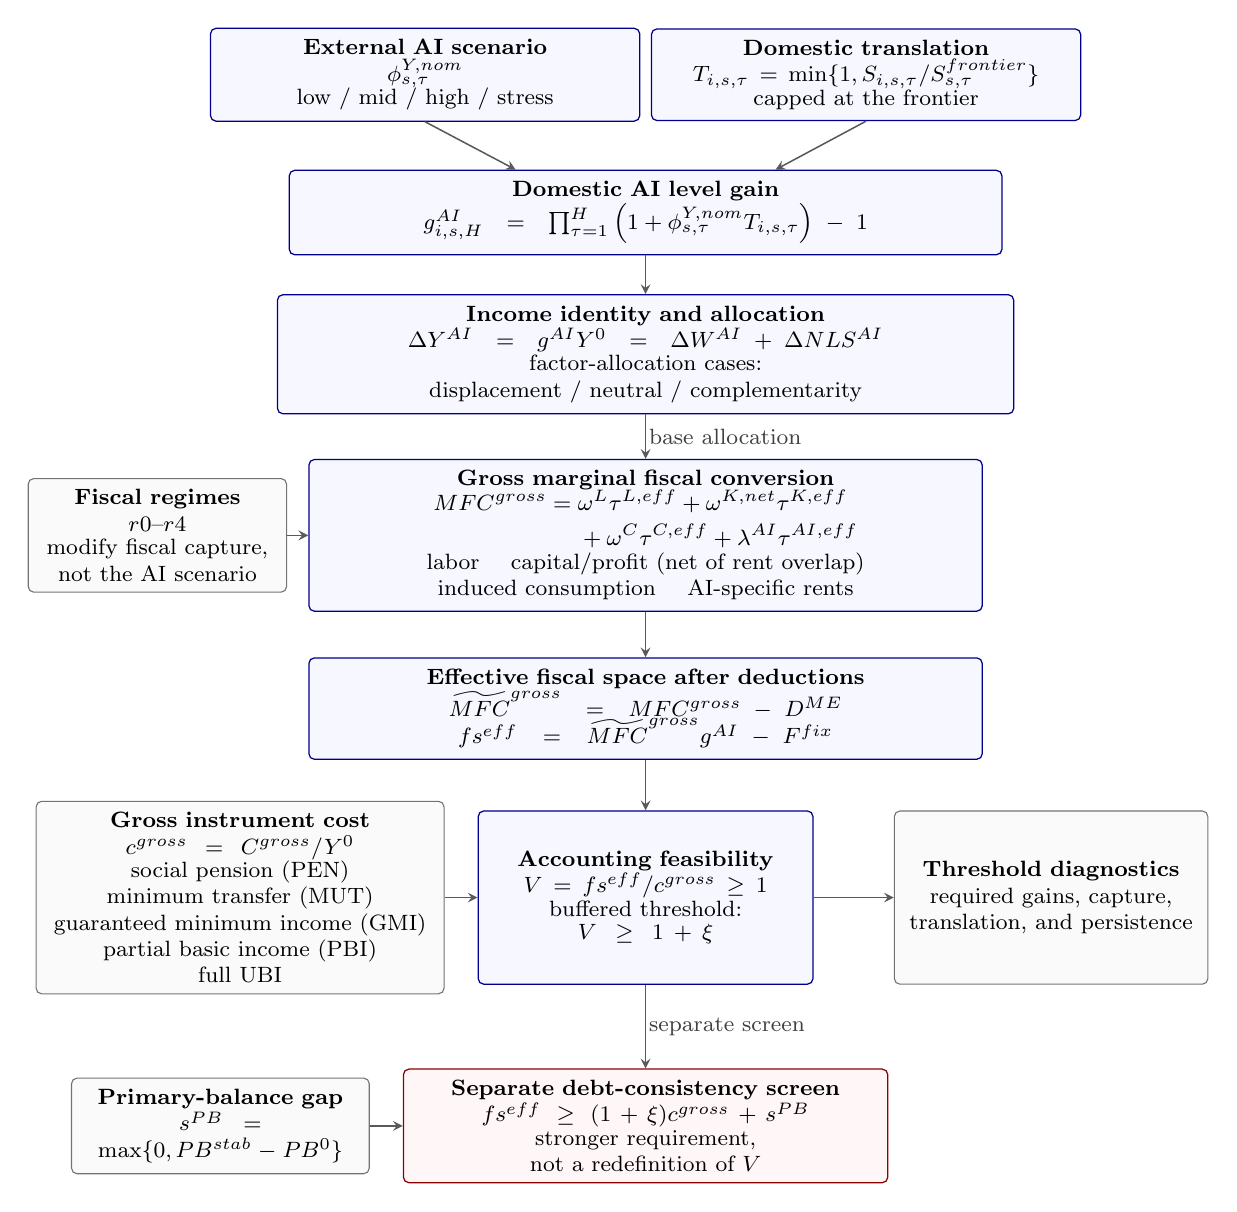
\begin{tikzpicture}[
  font=\footnotesize,
  mainbox/.style={draw=blue!55!black,fill=blue!3,rounded corners=2pt,
    line width=0.45pt,align=center,inner xsep=5pt,inner ysep=4pt},
  sidebox/.style={draw=black!55,fill=black!2,rounded corners=2pt,
    line width=0.4pt,align=center,inner xsep=4pt,inner ysep=4pt},
  debtbox/.style={draw=red!55!black,fill=red!3,rounded corners=2pt,
    line width=0.45pt,align=center,inner xsep=5pt,inner ysep=4pt},
  flow/.style={->,>=stealth,draw=black!65,line width=0.55pt},
  flowlabel/.style={font=\footnotesize,fill=white,inner sep=1pt,text=black!75}
]
  \node[mainbox,text width=5.1cm] (scenario) at (-2.8,0)
    {\textbf{External AI scenario}\\
     $\phi^{Y,nom}_{s,\tau}$\\[-1pt]
     {\footnotesize low / mid / high / stress}};
  \node[mainbox,text width=5.1cm] (translation) at (2.8,0)
    {\textbf{Domestic translation}\\
     $T_{i,s,\tau}=\min\{1,S_{i,s,\tau}/S^{frontier}_{s,\tau}\}$\\[-1pt]
     {\footnotesize capped at the frontier}};

  \node[mainbox,text width=8.7cm] (gain) at (0,-1.75)
    {\textbf{Domestic AI level gain}\\
     $g^{AI}_{i,s,H}=\prod_{\tau=1}^{H}
       \left(1+\phi^{Y,nom}_{s,\tau}T_{i,s,\tau}\right)-1$};
  \draw[flow] (scenario.south) -- ([xshift=-1.65cm]gain.north);
  \draw[flow] (translation.south) -- ([xshift=1.65cm]gain.north);

  \node[mainbox,text width=9.0cm] (identity) at (0,-3.55)
    {\textbf{Income identity and allocation}\\
     $\Delta Y^{AI}=g^{AI}Y^0=\Delta W^{AI}+\Delta NLS^{AI}$\\[-1pt]
     {\footnotesize factor-allocation cases:\\
      displacement / neutral / complementarity}};
  \draw[flow] (gain.south) -- (identity.north);

  \node[mainbox,text width=8.2cm] (mfc) at (0,-5.85)
    {\textbf{Gross marginal fiscal conversion}\\[-1pt]
     $\begin{aligned}
       MFC^{gross}={}&\omega^L\tau^{L,eff}+\omega^{K,net}\tau^{K,eff}\\[-2pt]
                    &+\omega^C\tau^{C,eff}+\lambda^{AI}\tau^{AI,eff}
     \end{aligned}$\\[-1pt]
     {\footnotesize labor \quad capital/profit (net of rent overlap)\\
      induced consumption \quad AI-specific rents}};
  \node[sidebox,text width=3.0cm] (regimes) at (-6.2,-5.85)
    {\textbf{Fiscal regimes}\\
     $r0$--$r4$\\[-1pt]
     {\footnotesize modify fiscal capture, not the AI scenario}};
  \draw[flow] (identity.south) -- node[flowlabel,right] {base allocation} (mfc.north);
  \draw[flow] (regimes.east) -- (mfc.west);

  \node[mainbox,text width=8.2cm] (space) at (0,-8.05)
    {\textbf{Effective fiscal space after deductions}\\
     $\widetilde{MFC}^{gross}=MFC^{gross}-D^{ME}$\\[-1pt]
     $fs^{eff}=\widetilde{MFC}^{gross}g^{AI}-F^{fix}$};
  \draw[flow] (mfc.south) -- (space.north);

  \node[sidebox,text width=4.9cm,minimum height=2.2cm] (cost) at (-5.15,-10.45)
    {\textbf{Gross instrument cost}\\
     $c^{gross}=C^{gross}/Y^0$\\[-1pt]
     {\footnotesize\hyphenpenalty=10000 social pension (PEN)\\
      minimum transfer (MUT)\\
      guaranteed minimum income (GMI)\\
      partial basic income (PBI)\\
      full UBI}};
  \node[mainbox,text width=3.9cm,minimum height=2.2cm] (threshold) at (0,-10.45)
    {\textbf{Accounting feasibility}\\
     $V=fs^{eff}/c^{gross}\geq1$\\[-1pt]
     {\footnotesize buffered threshold:\\[-1pt]
      $V\geq1+\xi$}};
  \node[sidebox,text width=3.7cm,minimum height=2.2cm] (diagnostics) at (5.15,-10.45)
    {\textbf{Threshold diagnostics}\\
     {\footnotesize required gains, capture,\\
      translation, and persistence}};
  \draw[flow] (space.south) -- (threshold.north);
  \draw[flow] (cost.east) -- (threshold.west);
  \draw[flow] (threshold.east) -- (diagnostics.west);

  \node[sidebox,text width=3.5cm] (pbgap) at (-5.4,-13.35)
    {\textbf{Primary-balance gap}\\
     $s^{PB}=\max\{0,PB^{stab}-PB^0\}$};
  \node[debtbox,text width=5.8cm] (debt) at (0,-13.35)
    {\textbf{Separate debt-consistency screen}\\
     $fs^{eff}\geq(1+\xi)c^{gross}+s^{PB}$\\[-1pt]
     {\footnotesize stronger requirement, not a redefinition of $V$}};
  \draw[flow] (threshold.south) -- node[flowlabel,right] {separate screen} (debt.north);
  \draw[flow] (pbgap.east) -- (debt.west);
\end{tikzpicture}
\end{singlespace}
\caption{Modular structure of the scenario-based threshold framework. An external AI scenario and domestic translation determine the domestic income gain, which is allocated across tax bases and converted into effective fiscal space. This space is compared with gross policy cost through the accounting threshold and, separately, with the stronger debt-consistency requirement. Arrows represent accounting mappings and comparisons, not causal effects.}
\label{fig:framework_chain}
\end{figure}

\subsection{From AI scenarios to domestic income}\label{subsec:scenario_translation}

The external scenario, $\phi^{Y,nom}_{s,\tau}$, is an annual AI-induced increment expressed in nominal-GDP-equivalent units. This bridge matters because task productivity, labor productivity, real output, and the nominal fiscal base are not interchangeable. The source evidence first enters in its reported unit and is then converted to the object used by the fiscal equations. The full unit bridges and parameter registry are documented in the replication package.

Domestic translation is summarized by $T_{i,s,\tau}\in[0,1]$. Let $S_{i,s,\tau}$ combine productive exposure, productive adoption, and absorptive capacity, and let $S^{frontier}_{s,\tau}$ denote the matching frontier benchmark. Translation and the resulting level gain are
\begin{align}
  T_{i,s,\tau}
    &=\min\left\{1,\frac{S_{i,s,\tau}}{S^{frontier}_{s,\tau}}\right\},
    \label{eq:translation_clean}\\
  g^{AI}_{i,s,H}
    &=\prod_{\tau=1}^{H}
      \left(1+\phi^{Y,nom}_{s,\tau}T_{i,s,\tau}\right)-1.
    \label{eq:level_gain_clean}
\end{align}
The frontier is drawn from the same reference population as the external scenario, so $T$ measures domestic translation rather than imposing a second adoption discount. Under a fixed annual scenario and fixed domestic structure, Equation~\eqref{eq:level_gain_clean} becomes $g^{AI}_{i,s,H}=(1+\phi^{Y,nom}_{s}T_{i,s})^H-1$.

The comparison is an endpoint annual-flow test. The accumulated level gain is interpreted as the increase in the recurring fiscal base available at horizon $H$, while policy costs are measured or projected for the same endpoint. It is not the sum of annual tax receipts and does not finance obligations incurred before the gain has accumulated. The translated gain is also additional domestic income, not yet public revenue. Fiscal conversion depends on how that income is distributed across taxable bases.

\subsection{From income allocation to fiscal space}\label{subsec:income_to_fiscal_space}

The domestic gain satisfies the functional-income identity
\begin{equation}
  \Delta Y^{AI}_{i,s}
  =g^{AI}_{i,s}Y_i^0
  =\Delta W^{AI}_{i,s}+\Delta NLS^{AI}_{i,s},
  \label{eq:income_identity_clean}
\end{equation}
where $\Delta W^{AI}$ is labor income and $\Delta NLS^{AI}$ is the non-labor residual. The latter includes mixed income, operating surplus, depreciation, rents, and other non-labor components; it is not synonymous with taxable corporate profit, especially where self-employment is extensive \citep{gollin2002getting}. Three allocation scenarios span the relevant incidence uncertainty. Under displacement, labor receives a smaller share of the increment; under neutral allocation, the pre-AI division is preserved; under complementarity, labor receives a larger share. These cases change composition only, not the accounting identity.

For fiscal channel $j$, the exposure ratio $\omega^j=(\Delta B^{j,tax}/Y^0)/g^{AI}$ measures the taxable base created per unit of domestic AI gain. Gross marginal fiscal conversion is
\begin{equation}
  MFC^{gross}_{i,s,r}
  =\omega^L_{i,s}\tau^{L,eff}_{i,s,r}
  +\omega^{K,net}_{i,s}\tau^{K,eff}_{i,s,r}
  +\omega^C_{i,s}\tau^{C,eff}_{i,s,r}
  +\lambda^{AI}_{i,s}\tau^{AI,eff}_{i,s,r}.
  \label{eq:mfc_clean}
\end{equation}
The four terms capture labor income, taxable capital and profit income net of any AI-rent overlap, induced taxable consumption, and AI-specific rents. Effective rates incorporate the relevant compliance and capturability adjustments. The $\omega$ terms are base-response ratios, not probability weights, and need not sum to one. Informality is assigned either to a taxable base or to its effective rate, while AI rents are treated either as a subset of the capital base or as an additional base. Appendix~\ref{app:conventions} records these conventions in one table. This channel construction allows fiscal regimes to alter capture without changing the underlying technology scenario, following the policy channels emphasized by \citet{brollo2024fiscal}.

Let $D^{ME}_{i,s,r}$ collect administrative, transition, and residual-leakage deductions expressed per unit of the AI gain, and let $F^{fix}_{i,p,s,r}$ collect their fixed GDP-share counterparts. Each component enters one margin. Net marginal capture and effective fiscal space are
\begin{align}
  \widetilde{MFC}^{gross}_{i,s,r}
    &=MFC^{gross}_{i,s,r}-D^{ME}_{i,s,r},
    \label{eq:mfc_tilde_clean}\\
  fs^{eff}_{i,p,s,r}
    &=\widetilde{MFC}^{gross}_{i,s,r}g^{AI}_{i,s}-F^{fix}_{i,p,s,r}.
    \label{eq:fiscal_space_clean}
\end{align}

Historical experience disciplines this constructed capture rate without being added to it. The gross historical benchmark is
\begin{equation}
  MFC^{hist,gross}_{i,t}
  =\frac{\Delta \mathrm{Revenue}_{i,t}}{\Delta \mathrm{GDP}_{i,t}}.
  \label{eq:mfc_historical_clean}
\end{equation}
Comparing gross channel-based capture with the country's historical gross-capture distribution distinguishes ordinary requirements from historically demanding ones. It also keeps plausibility separate from feasibility: a cell can satisfy the accounting threshold while relying on an unusual fiscal response, or fail despite a historically ordinary conversion rate. Once effective fiscal space is constructed, feasibility depends on the cost of the instrument it is asked to finance.

\subsection{Policy costs, feasibility, and diagnostic inversions}\label{subsec:feasibility_inversions}

For eligible units $u\in\mathcal U_{i,p}$ with weights $w_u$ and benefits $B_{u,i,p}$, the generic gross cost and the canonical feasibility ratio are
\begin{align}
  C^{gross}_{i,p}
    &=\sum_{u\in\mathcal U_{i,p}}w_uB_{u,i,p},
  &c^{gross}_{i,p}
    &=\frac{C^{gross}_{i,p}}{Y_i^0},
    \label{eq:policy_cost_clean}\\
  V^{gross}_{i,p,s,r}
    &=\frac{fs^{eff}_{i,p,s,r}}{c^{gross}_{i,p}},
  &V^{gross}_{i,p,s,r}&\geq1.
    \label{eq:viability_clean}
\end{align}
The empirical application prices a social pension, a minimum transfer, a guaranteed minimum income, a partial basic income, and a full UBI benchmark under this common denominator. Gross cost is the primary comparison, which prevents uncertain spending offsets from creating a mechanical crossing. Hereafter $V$ denotes $V^{gross}$. The threshold $V=1$ means exact accounting coverage; a prudential buffer $\xi\geq0$ requires $V\geq1+\xi$. This is a financing screen, not a welfare, political, administrative, or full debt-sustainability criterion \citep{imf2016fiscalspace}.

Debt consistency is imposed as a separate guardrail. Let $PB_i^0$ be the baseline primary balance and $PB_i^{stab}$ the balance that stabilizes debt under the maintained macroeconomic path. Define
\begin{align}
  s_i^{PB}
    &=\max\{0,PB_i^{stab}-PB_i^0\},
    \label{eq:primary_balance_gap_clean}\\
  fs^{eff}_{i,p,s,r}
    &\geq(1+\xi)c^{gross}_{i,p}+s_i^{PB},
    \label{eq:debt_guardrail_clean}\\
  \mathcal R_{i,p,s,r}(\xi)
    &=(1+\xi)c^{gross}_{i,p}+F^{fix}_{i,p,s,r},
  &\mathcal R^{DC}_{i,p,s,r}(\xi)
    &=\mathcal R_{i,p,s,r}(\xi)+s_i^{PB}.
    \label{eq:requirements_clean}
\end{align}
The first requirement asks whether AI-induced fiscal space covers the instrument. The debt-consistent requirement asks whether it also closes any inherited primary-balance shortfall. It is deliberately a stronger test, rather than a redefinition of the accounting threshold.

Figure~\ref{fig:frontier_clean} gives the threshold geometry, writing $\widetilde M$ for $\widetilde{MFC}^{gross}$. For fixed requirements, higher domestic gains compensate for lower marginal capture and conversely. A larger policy cost, prudential buffer, fixed deduction, or primary-balance gap shifts the boundary outward. The figure replaces a separate formal construction of the frontier.

\begin{figure}[H]
\centering
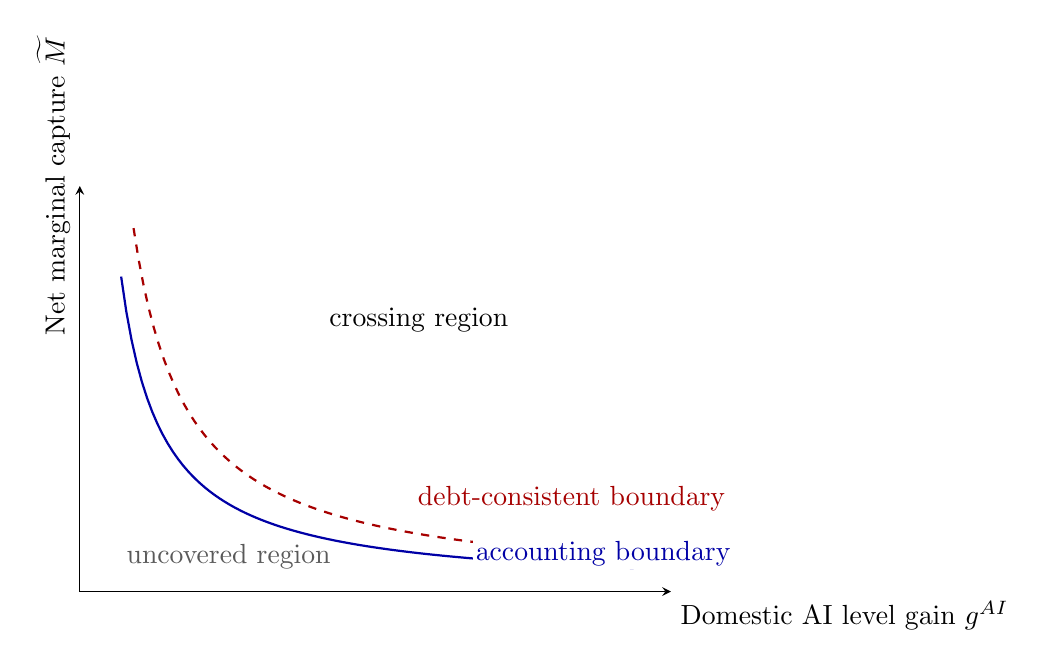
\begin{tikzpicture}[x=1.05cm,y=1.0cm,>=stealth]
  \draw[->] (0,0) -- (7.15,0)
    node[below right,align=center] {Domestic AI level gain $g^{AI}$};
  \draw[->] (0,0) -- (0,5.15)
    node[above left,rotate=90,anchor=south] {Net marginal capture $\widetilde M$};
  \draw[thick,blue!65!black,domain=0.5:6.7,samples=100]
    plot (\x,{2.0/\x});
  \draw[thick,dashed,red!65!black,domain=0.65:6.7,samples=100]
    plot (\x,{3.0/\x});
  \node[blue!65!black,anchor=west,fill=white,inner sep=1pt] at (4.75,0.48)
    {accounting boundary};
  \node[red!65!black,anchor=west,fill=white,inner sep=1pt] at (4.05,1.18)
    {debt-consistent boundary};
  \node[align=center] at (4.1,3.45) {crossing region};
  \node[align=center,text=gray!70!black] at (1.8,0.45) {uncovered region};
\end{tikzpicture}
\caption{Schematic feasibility boundaries. The solid curve satisfies
$\widetilde M g^{AI}=\mathcal R(\xi)$; combinations above it cross the buffered accounting threshold. The dashed curve adds the primary-balance correction, $\widetilde M g^{AI}=\mathcal R^{DC}(\xi)$. The axes are not drawn to empirical scale.}
\label{fig:frontier_clean}
\end{figure}

The same identities can be inverted to report requirements rather than a binary outcome. Suppressing indices and letting $\mathcal R$ denote either the accounting or debt-consistent requirement,
\begin{align}
  g^{AI,*}
    &=\frac{\mathcal R}{\widetilde{MFC}^{gross}},
  &MFC^{gross,*}
    &=\frac{\mathcal R}{g^{AI}}+D^{ME},
    \label{eq:g_mfc_inversions_clean}\\
  T^{req,H}
    &=\frac{\left(1+\mathcal R/\widetilde{MFC}^{gross}\right)^{1/H}-1}
            {\phi^{Y,nom}}.
    \label{eq:translation_inversion_clean}
\end{align}
These quantities answer how large the domestic gain, gross fiscal capture, or translation factor would have to be. The closed forms hold with channel weights fixed at the evaluated scenario, and the translation formula uses a constant annual scenario and domestic structure over $H$. Recomputing taxable-base composition as the shock changes, or allowing a time-varying path, turns the corresponding inversion into a numerical root. Appendix~\ref{app:derivations} provides the derivations. Since $T\leq1$, a requirement above one lies beyond the domestic-translation frontier. This diagnosis does not by itself make translation the sole constraint: several required margins can exceed their admissible or historically supported ranges at the same time.

The temporal inversion holds the scenario and domestic structure fixed and asks how long the annual translated increment would need to persist:
\begin{equation}
  H^*_{i,p,s,r}(\xi)
  =\min\left\{
    H\in\mathbb N:
    \widetilde{MFC}^{gross}_{i,s,r}
    \left[\left(1+\phi^{Y,nom}_{s}T_{i,s}\right)^H-1\right]
    \geq(1+\xi)c^{gross}_{i,p}(H)+F^{fix}_{i,p,s,r}
  \right\}.
  \label{eq:hstar_clean}
\end{equation}
The debt-consistent version adds $s_i^{PB}$ to the right-hand side. Endpoint costs may vary with the eligible population, which is why $c^{gross}(H)$ remains inside the definition. $H^*$ is a required persistence horizon, not a forecast date. It was introduced after the baseline as a derived reporting extension; it changes no calibrated input and no baseline classification.

Section~\ref{sec:design} maps these objects into country data, policy-cost rules, AI scenarios, fiscal regimes, and calibrated uncertainty.

\section{Empirical Design}\label{sec:design}

The accounting objects in Section~\ref{sec:framework} are taken to data through a calibrated empirical-simulation design. The unit of analysis is a country--policy--AI-scenario--fiscal-regime cell. This structure holds the technological scenario apart from the fiscal regime, so that changes in domestic translation, policy cost, and public capture can be read separately without treating their contrasts as causal estimates. It also permits joint shortfalls: a cell may require both more domestic translation and more fiscal capture than the calibrated supports allow. The design therefore does not assign failure to a single margin by construction. The primary channel construction and calibrated supports were prespecified.

\subsection{Country anchors and data}\label{subsec:country_data_clean}

The application covers Peru, Chile, Colombia, and Mexico. All four economies use a common 2024 harmonization anchor, a ten-year accumulation horizon, and a 2034 endpoint. Structural inputs are held at their harmonized anchor values over the accumulation period; the endpoint exception is the eligible-population share used to price demographically defined programs. Earlier observations needed for slow-moving anchors are carried to the common year with their provenance retained in the replication package.\footnote{The archived package is available at \url{https://doi.org/10.5281/zenodo.21348535}.}

The macro-fiscal block combines WDI national accounts and population data, OECD Revenue Statistics and IMF fiscal series, and the UNU-WIDER Government Revenue Dataset for historical comparison. PIP supplies the aggregate poverty measures. UN World Population Prospects supplies endpoint demographic shares; PWT supplies the labor-share anchor; IMF AIPI, ITU, and Ookla supply preparedness and digital-access inputs; and national official sources determine social-pension rules \citep{worldbank2026wdi,worldbank2026pip,oecd2025revenue,unu2025grd,unwpp2024,pwt1001,imf2024aipi,itu2026datahub,ookla2024speedtest}. Table~\ref{tab:country_data_clean} distinguishes the official aggregate grid from the household-data extensions.

The common year makes the cross-country accounting comparable but does not turn the sample into a regional panel. The four economies were chosen to span different combinations of preparedness, informality, social-policy architecture, and fiscal capacity; the application is deliberately comparative rather than representative of Latin America. Fiscal variables are aligned to a consistent government concept within country. Historical revenue capture remains an external plausibility benchmark, while the channel-based construction in Equation~\eqref{eq:mfc_clean} supplies the primary regime comparisons.

\begin{table}[H]
\centering
\small
\caption{Country and household-data coverage}
\label{tab:country_data_clean}
\begin{tabular}{@{}l>{\raggedright\arraybackslash}p{0.27\textwidth}>{\raggedright\arraybackslash}p{0.54\textwidth}@{}}
\toprule
Country & Design anchor & Household-data role \\
\midrule
Peru & 2024 harmonized inputs & Aggregate PIP cost in the official grid; ENAHO 2024 GMI extension. \\
Chile & 2024 harmonized inputs & Aggregate PIP cost in the official grid; CASEN 2024 GMI extension. \\
Colombia & 2024 harmonized inputs & Aggregate inputs; no household-microdata extension in the archived design. \\
Mexico & 2024 harmonized inputs & Aggregate inputs; no household-microdata extension in the archived design. \\
\bottomrule
\end{tabular}
\end{table}

The household surveys are validation extensions rather than inputs to the official four-country grid. The Peru extension uses the ENAHO 2024 Sumaria file \citep{inei2024enaho}. Its row-level microdata are treated as restricted for redistribution: the public replication package provides retrieval instructions, code, hashes, and aggregate outputs, but does not redistribute the source file. The Chile extension analogously uses CASEN 2024 \citep{mdsf2024casen}. Official comparisons therefore retain aggregate GMI costs, with the survey estimates serving as separately identified validation extensions.

\subsection{Policy instruments and endpoint costs}\label{subsec:policy_costs_clean}

Five policy concepts are priced under the common gross-cost denominator in Equation~\eqref{eq:policy_cost_clean}: a social pension (PEN), a minimum universal transfer (MUT), a guaranteed minimum income (GMI), a partial basic income for adults (PBI), and a full universal basic income benchmark (UBI). PEN preserves each country's official eligibility and benefit schedule. MUT supplies a low common transfer benchmark; GMI closes an aggregate poverty gap; PBI supplies a partial adult grant; and UBI is retained as the fiscally demanding universal benchmark.

The five concepts generate six reported cost rows because GMI is priced twice. \nolinkurl{GMI_ideal_aggregate} applies ideal targeting to the grouped PIP poverty gap and is therefore a mechanical lower-cost case. \nolinkurl{GMI_loaded_aggregate} applies the fixed targeting-cost loading to the same aggregate gap. Carrying both variants into every comparison prevents a favorable targeting convention from standing in for the instrument itself. These are two aggregate-cost variants, not two household microsimulations.

Costs and AI-induced fiscal space are evaluated at the same endpoint and against the same no-AI GDP denominator. For instruments whose eligibility is demographic, the 2024 gross-cost ratio is scaled to 2034 by the policy-specific WPP eligible-share ratio,
\begin{equation}
  c^{gross}_{i,p,2034}
  =c^{gross}_{i,p,2024}
   \frac{e^{WPP}_{i,p,2034}}{e_{i,p,2024}}.
  \label{eq:endpoint_cost_clean}
\end{equation}
The eligible-share definition follows the policy rule, including the sex- and age-specific schedule for Colombia's pension. For aggregate GMI, the primary design freezes the poverty distribution, so $c^{gross}_{i,GMI,2034}=c^{gross}_{i,GMI,2024}$. Appendix~\ref{app:conventions} records, once, the treatment of existing spending, administrative costs, informality, and AI rents.

This pricing convention treats each instrument as a recurring annual commitment at the endpoint. The gross-cost comparison does not presume that an existing program can be discontinued or that transfer spending immediately returns as tax revenue. Policy-specific administration, transition, and leakage terms enter the fiscal-space side of the comparison defined in Section~\ref{sec:framework}. Net-cost and alternative implementation assumptions remain sensitivity exercises, so the primary ranking reflects program scale rather than an assumed financing offset.

\subsection{AI scenarios and fiscal regimes}\label{subsec:scenarios_regimes_clean}

The four AI scenarios enter only after the source unit has been bridged to the annual nominal-GDP-equivalent object used in Equation~\eqref{eq:level_gain_clean}. Table~\ref{tab:scenario_inputs_clean} reports the deterministic model-ready inputs. Low and moderate are TFP-equivalent cases. High begins as a frontier labor-productivity input \citep{oecd2025g7}, so its country-specific labor-productivity-to-GDP bridge places the final input between 0.306 and 0.421 percent per year. It consequently lies below the 0.425 percent moderate input for all four economies after the bridge. The labels identify source cases, not an imposed ordinal ranking after conversion. The disruptive 1.5 percent case is a diagnostic stress test deliberately outside the macroeconomic literature used to discipline the lower cases; it is not a forecast.

\begin{table}[H]
\centering
\small
\caption{Annual model-ready AI scenario inputs}
\label{tab:scenario_inputs_clean}
\begin{tabular}{@{}l>{\raggedright\arraybackslash}p{0.25\textwidth}>{\raggedright\arraybackslash}p{0.48\textwidth}@{}}
\toprule
Scenario & $\phi^{Y,nom}$ (percent) & Interpretation \\
\midrule
Low & 0.050 & Low TFP-equivalent case. \\
Moderate (mid) & 0.425 & Central TFP-equivalent case. \\
Frontier input (high) & 0.306--0.421 & Labor-productivity frontier after the country bridge. \\
Disruptive (stress) & 1.500 & Diagnostic stress case, not a forecast. \\
\bottomrule
\end{tabular}
\begin{minipage}{0.94\textwidth}\footnotesize
\emph{Note:} Scenario labels denote source cases, not an ordinal ranking of the model-ready input; after the labor-productivity-to-GDP bridge, the frontier (high) input lies below the moderate TFP-equivalent input in all four economies.
\end{minipage}
\end{table}

Fiscal regimes change marginal capture, not the technological scenario. \texttt{r0} holds observed effective rates at the status quo. \texttt{r1} represents improved compliance, and \texttt{r2} broadens tax bases. \texttt{r3} introduces explicit tax treatment of AI rents: the rents are separated from the ordinary capital base and assigned a lower effective rate, with the behavioral-erosion companion. \texttt{r4} combines the reform margins. This construction does not mechanically raise total marginal capture; in the evaluated calibration, median $MFC^{gross}$ is lower under \texttt{r3} than under \texttt{r0}. The reform cases operate through channel-specific effective rates and the corresponding base margins, and all are paired with behavioral erosion that reduces the taxable base as effective rates rise. This makes the mechanical reform case an upper comparison while leaving the AI gain itself unchanged. Because scenario and regime are crossed rather than bundled, the threshold inversions can reveal whether neither frontier translation nor stronger fiscal capture is sufficient in a given cell.

\subsection{Calibrated uncertainty and crossing frequencies}\label{subsec:uncertainty_clean}

Unobserved primitives with specified lower, central, and upper values receive bounded PERT distributions; a degenerate support is treated as fixed. The simulation draws primitives for the scenario, domestic translation, policy cost, and fiscal-conversion channels, then derives $T$, $g^{AI}$, $MFC^{gross}$, and $V^{gross}$. Drawing primitives rather than those derived objects preserves the accounting links across modules within each realization. The primary grid uses 5,000 draws per cell. Selected baseline cells are rerun at 10,000, 25,000, and 50,000 draws to assess numerical convergence. Independent blocks provide the transparent primary specification, while signed rank-correlated institutional-factor designs test dependence among preparedness, informality, adoption, exposure, and fiscal bases.

For prudential margin $\xi$, the reported quantity is
\begin{equation}
  \widehat{\pi}_{i,p,s,r}(\xi)
  =\frac{1}{M}\sum_{m=1}^{M}
   \mathbf{1}\!\left\{V^{gross,(m)}_{i,p,s,r}\geq1+\xi\right\}.
  \label{eq:crossing_frequency_clean}
\end{equation}
The quantity $\widehat{\pi}$ is interpreted as a model-implied crossing frequency across calibrated draws, not as a predictive probability. It is conditional on the selected parameter supports, distributional forms, and dependence assumptions. More draws reduce simulation error relative to that calibrated distribution; they do not establish correspondence with realized uncertainty.

\subsection{Diagnostic and robustness strategy}\label{subsec:diagnostics_design_clean}

The ICT-era temporal placebo provides the falsification exercise: it reanchors the reduced-form calculation to 2010--2018 using the recorded digital-access proxy, historical fiscal capture, and era-proximate policy-cost anchors, testing whether ordinary digitalization is mechanically relabeled as fiscal space. The reduced-form exposure-rescaling diagnostic then substitutes automation-risk exposure for productive exposure at the ratio level,
\begin{equation}
  V^{NC}_{i,p,s,r}
  =V^{gross}_{i,p,s,r}\frac{E^{auto}_{i}}{E^{prod}_{i}}.
  \label{eq:negative_control_clean}
\end{equation}
This operation does not re-estimate $T$ by sector. It follows the diagnostic logic of negative controls but, because it only rescales $V$, is not a complete negative-control design and supplies no causal estimand \citep{lipsitch2010negative}. Channel leave-one-out exercises remove each fiscal-conversion channel in turn, with companion checks for AI-rent capture and adoption-side informality. A limited leave-one-source-out check replaces the OECD revenue anchor with the comparable GRD measure where a like-for-like general-government alternative exists; source-unique inputs are reported as unavailable rather than imputed. Appendix~\ref{app:robustness_design} summarizes these operations. The next section reports their results alongside the threshold, debt, persistence, and crossing-frequency evidence.

\section{Results}\label{sec:results}

\subsection{Policy costs and the joint non-stress shortfall}\label{subsec:results_costs_shortfall}

Under the primary channel-based specification, no deterministic crossing occurs in the non-stress scenarios (low, mid, or frontier). The first reason is scale: the common denominator makes clear that the same policy label can imply very different commitments across settings. Table~\ref{tab:costs_results_clean} reports the six cost rows generated by the five instruments. Full UBI is the largest commitment everywhere, at 11.62--21.36 percent of endpoint GDP, followed by PBI at 4.85--7.97 percent. The relative position of the cheaper instruments is country-specific. Social pensions cost 0.56 percent of GDP in Peru but 3.10 percent in Chile, reflecting national benefit and eligibility rules. Ideal GMI costs only 0.15 percent in Chile, compared with 2.99 percent in Colombia; the loaded variant raises the cost in every country. A policy-cost gradient is therefore visible at broad scale, but there is no universal ordering among pensions, MUT, and GMI.

\begin{table}[H]
\centering
\small
\begin{singlespace}
\caption{Comparable gross policy costs (percent of endpoint GDP)}
\label{tab:costs_results_clean}
\begin{tabular}{@{}lrrrr@{}}
\toprule
Instrument & Chile & Colombia & Mexico & Peru \\
\midrule
Social pension (PEN) & 3.10 & 0.90 & 1.60 & 0.56 \\
Minimum universal transfer (MUT) & 2.90 & 4.75 & 3.95 & 5.34 \\
GMI, ideal targeting & 0.15 & 2.99 & 1.01 & 2.79 \\
GMI, loaded targeting & 0.22 & 4.48 & 1.52 & 4.18 \\
Partial basic income (PBI) & 4.85 & 7.43 & 5.91 & 7.97 \\
Full UBI benchmark & 11.62 & 18.98 & 15.81 & 21.36 \\
\bottomrule
\end{tabular}
\begin{minipage}{0.94\textwidth}\footnotesize
\emph{Note:} GMI costs are fixed aggregate endpoint costs; demographic instruments use the fixed endpoint eligible-share rule. Gross and net columns coincide because the primary comparison credits no existing-spending offset.
\end{minipage}
\end{singlespace}
\end{table}


The table is a financing comparison, not a ranking of social value. A low cost can reflect narrow eligibility, a low benefit, a small measured poverty gap, or ideal targeting; it does not establish adequacy or administrative desirability. Conversely, the UBI row is retained because its universal denominator makes it a useful fiscal stress benchmark, not because it is the preferred policy in every country. Keeping gross cost in the primary comparison also prevents assumed program replacement from mechanically improving $V$. Any credit for substitutable existing spending belongs to a labeled sensitivity rather than to the cross-instrument ranking.

The household extensions support using the aggregate GMI rows without making them appear exact. At the matched international poverty threshold, the primary CASEN estimate is 0.39 percent above Chile's aggregate GMI cost. The corresponding ENAHO estimate is 7.73 percent below Peru's aggregate cost. In both cases the loaded version inherits the same relative difference because it applies the same targeting-cost factor. These comparisons validate the order of magnitude while leaving the official four-country grid on its common aggregate basis.

The second reason is that the domestic gain and fiscal conversion are jointly too small. Across all 360 low, mid, and high cells, no value reaches the structural accounting threshold. The largest is $V^{gross}=0.177$, for Peru's social pension under the mid scenario and r4. The high frontier input does not overturn this result; as explained in Section~\ref{subsec:scenarios_regimes_clean}, its country bridge can place it below the mid input after conversion. The absence of a high-scenario crossing is therefore a result of the model-ready inputs, not an imposed monotonic scenario ordering.

The diagnostic inversions show why the shortfall should not be assigned to one margin. With the 10-percent prudential buffer, every mid-scenario accounting and debt-consistent cell requires $T^{req,H}>1$. The smallest requirement is 1.0941, for Chile's ideal GMI under r4, already beyond the domestic-translation frontier. Holding that cell's translation fixed instead, the minimum required AI-rent capture rate is 202.46 percent. This is 13.50 times the most permissive specified upper support of 15 percent under r4. Thus frontier translation alone does not close the gap, and neither does capture at the strongest specified reform setting. Panel B of Table~\ref{tab:frequency_threshold_hstar_clean} shows that the required domestic gain and gross marginal fiscal conversion also rise sharply for the corresponding Peruvian, Colombian, and Mexican instruments. The mid-scenario result is a joint shortfall in translated income and public capture. Because productive exposure uses a common LAC fallback, cross-country translation differences in the evaluated grid operate through preparedness and adoption; the design does not separately identify a country-specific productive-exposure gradient.

Some low-scenario values are negative because fixed administration, transition, and leakage deductions exceed the small revenue flow generated by the translated gain. This does not imply that AI reduces output in those cells; it means that the incremental fiscal-space numerator is negative after implementation costs. As the scenario strengthens, reform raises marginal conversion and the fixed deductions become less important relative to the gain. Yet the best mid cell remains far below coverage, so the result is not a knife-edge consequence of one small fixed-cost assumption.

\subsection{Stress crossings and the debt guardrail}\label{subsec:results_stress_debt}

Only the disruptive stress scenario produces deterministic accounting crossings, and the debt guardrail separates Chile's GMI result from Peru's pension result. Figure~\ref{fig:headline_feasibility_clean} displays the r0 grid on a common categorical scale. It makes three features visible at once: there is no crossing in the lower three scenario columns; both Chilean GMI cost variants cross under stress; and Peru's pension crossing is marginal relative to the prudential buffer.

\begin{figure}[H]
\centering
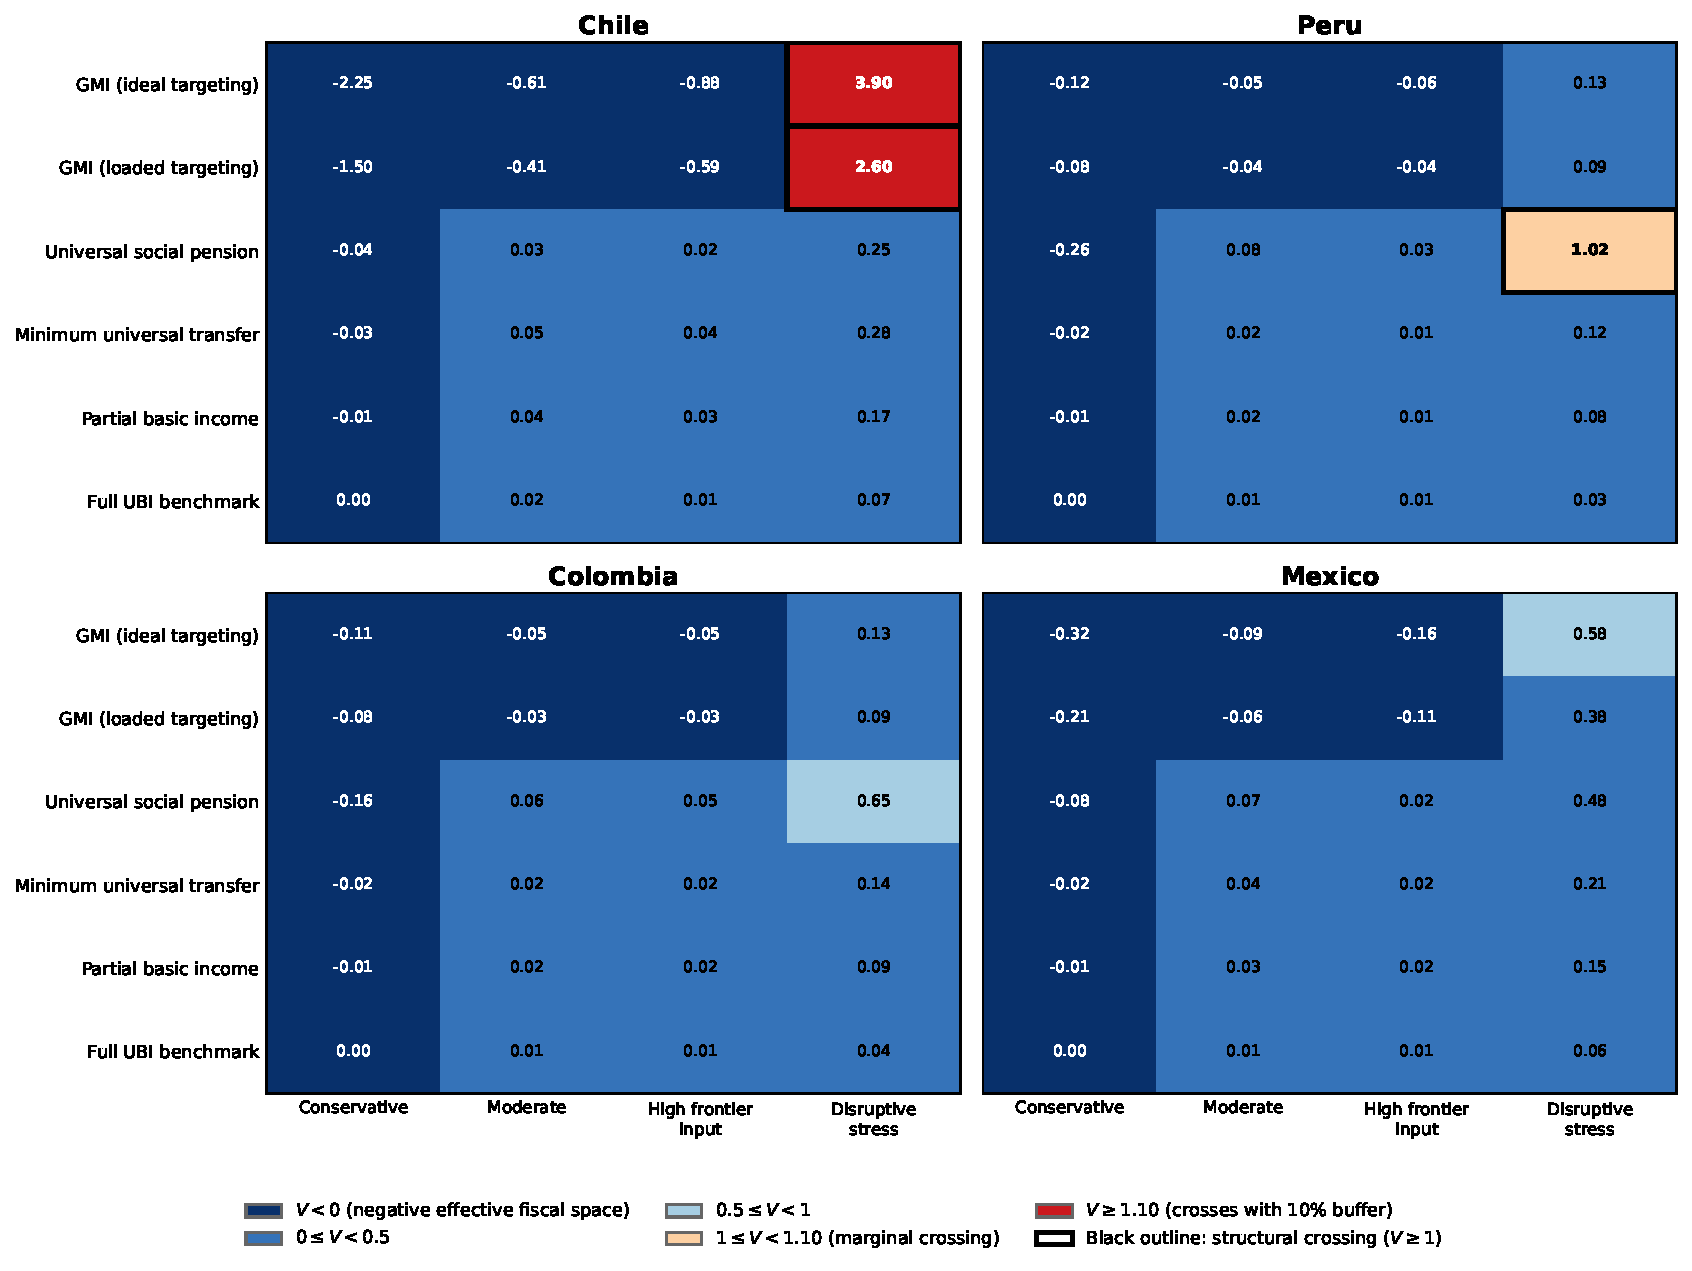
\includegraphics[width=\textwidth]{figures/headline_feasibility.pdf}
\caption{Primary feasibility grid under the status-quo fiscal regime. Each entry is deterministic $V^{gross}$ from the primary grid, rounded to two decimals. The black outline marks the structural accounting threshold $V\geq1$; the categorical fill distinguishes cells below zero, below one, between 1 and 1.10, and at or above the 10-percent prudential buffer.}
\label{fig:headline_feasibility_clean}
\end{figure}

Under r0, Chile's ideal GMI reaches $V=3.90$ and its loaded companion reaches $V=2.60$. Both pass the debt guardrail, and both remain debt-consistent across r0--r4. Combined reform raises the corresponding values to 5.80 and 3.87. The loaded result matters because it shows that the crossing is not created by ideal targeting alone. Its interpretation is nevertheless conditional: it requires persistence of the disruptive scenario that the design treats as a diagnostic stress test, not as a central macroeconomic projection.

Peru's social pension also crosses the structural accounting threshold under stress in every regime, with $V$ ranging from 1.02 to 1.42. Only r2 and r4 also clear $V=1.10$. More importantly, none closes the inherited primary-balance gap: every row is classified as accounting feasible but debt failed. The result is therefore fragile in a fiscal sense even where reform increases contemporaneous coverage. Colombia and Mexico never reach the accounting threshold. Their strongest stress cells are Colombia's pension under r4, at 0.91, and Mexico's ideal GMI under r4, at 0.80. Table~\ref{tab:deterministic_results_clean} collects these classifications.

The guardrail is doing distinct work here. It does not reprice the transfer or reduce the AI-induced revenue flow; it asks whether that flow can finance the policy while also covering the primary-balance correction inherited from the maintained debt path. A structural crossing can therefore remain informative as an accounting result and still be insufficient as a fiscal commitment. That distinction is why the Chile and Peru stress rows should not be grouped under a single feasibility label.

\begin{table}[H]
\centering
\small
\begin{singlespace}
\caption{Selected deterministic outcomes and the debt guardrail}
\label{tab:deterministic_results_clean}
\begin{tabular}{@{}>{\raggedright\arraybackslash}p{0.31\textwidth}>{\raggedright\arraybackslash}p{0.16\textwidth}r >{\raggedright\arraybackslash}p{0.34\textwidth}@{}}
\toprule
Scope or cell & Reported regime & $V^{gross}$ & Result class \\
\midrule
All low/mid/high cells & Best of 360 cells & 0.177 & No accounting crossing \\
Chile, GMI ideal, stress & r0 & 3.90 & Feasible, including debt guardrail \\
Chile, GMI loaded, stress & r0 & 2.60 & Feasible, including debt guardrail \\
Peru, social pension, stress & r0--r4 & 1.02--1.42 & Accounting crossing; debt guardrail fails \\
Colombia, best cell (PEN, stress) & r4 & 0.91 & No accounting crossing \\
Mexico, best cell (GMI ideal, stress) & r4 & 0.80 & No accounting crossing \\
\bottomrule
\end{tabular}
\begin{minipage}{0.94\textwidth}\footnotesize
\emph{Note:} Accounting crossings use the structural threshold $V\geq1$; Figure~\ref{fig:headline_feasibility_clean} separately identifies cells that also reach $V\geq1.10$. Stress is a diagnostic scenario, not a forecast.
\end{minipage}
\end{singlespace}
\end{table}


The deterministic evidence consequently supports a narrow hierarchy of findings. Chilean GMI is conditionally feasible only under diagnostic stress; Peru's pension has an accounting crossing without debt consistency; and neither Colombia nor Mexico has a crossing in the evaluated grid. Reform changes the distance to the threshold, but it does not turn a lower AI scenario into a feasible cell.

\subsection{Crossing frequencies, threshold requirements, and persistence}\label{subsec:results_mc_hstar}

Calibrated uncertainty reinforces the conditional nature of the deterministic crossings. In the primary channel Monte Carlo, the largest model-implied frequency over low, mid, and high scenarios is 2.36 percent, again for Chile's ideal GMI under mid and r4. Allowing the specified factor-dependence structures raises the maximum to 4.44 percent, without changing the absence of a deterministic non-stress crossing. These are frequencies across calibrated draws, not predictive probabilities; their scale is conditional on the parameter supports, distributional forms, and dependence design described in Section~\ref{subsec:uncertainty_clean}.

The historical reduced-form modes produce a deliberately different result. Historical increment ratios embed discretionary tax changes, commodity cycles, crisis recoveries, denominator noise, and shifts in revenue composition; they serve as reduced-form robustness benchmarks rather than as the preferred estimate of marginal capture from an AI-specific increment. For Chile's GMI under mid and r0, drawing gross capture from the historical distributions gives crossing frequencies of 66.06--91.76 percent for ideal GMI and 55.78--85.10 percent for loaded GMI. These modes are available only under r0 and replace the channel construction with a historical-capture draw; they do not show that the primary channel model predicts a likely mid-scenario crossing. Rather, the contrast identifies fiscal conversion as an empirically consequential modeling choice. The total-revenue variants occupy the upper part of these ranges, while the tax-based mixtures are lower.

Under stress, Chilean GMI has primary channel frequencies of 94.78--99.98 percent across its two cost variants and five regimes, with the debt-consistent frequency unchanged. Peru's pension is different: its accounting crossing frequency ranges from 41.02 to 80.50 percent, but the debt-consistent frequency is only 0.02--2.48 percent. The latter upper value occurs under r4; it is small, but not below one percent. Panel A of Table~\ref{tab:frequency_threshold_hstar_clean} keeps the primary, dependence, and historical objects separate.

This comparison also clarifies why a deterministic crossing is not a probability statement. The point calibration fixes one value for every primitive, whereas the simulation draws the scenario, translation, policy cost, and fiscal channels jointly within their stated supports. Chile's stress result remains well inside the crossing region across most draws. Peru's accounting result lies nearer the boundary, so its frequency is more responsive to the fiscal regime, and the debt correction moves almost the entire calibrated distribution back below the stronger requirement.

The inversion panel turns these crossing frequencies into requirements. Chile's ideal GMI under mid and r4 is the closest non-stress cell, while Peru's pension, Colombia's pension, and the Mexican GMI variants require progressively larger accumulated gains and gross fiscal conversion. In every listed row the required translation exceeds one, and the AI-rent inversion lies outside a feasible tax-rate domain. The exercise therefore reports how far each cell is from the boundary rather than treating every non-crossing as equivalent.

The persistence inversion gives the same comparison in years, but it is a post-baseline derived extension. At the 10-percent buffer, Chile's ideal GMI under stress requires six years of persistence under r0 and five under r4; the debt-consistent horizon is the same. Peru's pension has an accounting horizon of 8--11 years, but the debt-consistent requirement is 17--22 years. Colombia's pension reaches the accounting boundary in 13--19 years, while its debt-consistent counterpart is censored beyond 25 years. Mexico's ideal GMI requires 13--16 years and its loaded GMI 17--21 years on the accounting basis; both debt-consistent versions are likewise beyond 25 years. These are conditional persistence requirements, not calendar forecasts or expected adoption dates.

\begin{table}[H]
\centering
\footnotesize
\begin{singlespace}
\caption{Crossing frequencies, threshold requirements, and persistence horizons}
\label{tab:frequency_threshold_hstar_clean}
\textit{Panel A. Model-implied crossing frequencies across calibrated draws}\\[0.2em]
\begin{tabular}{@{}>{\raggedright\arraybackslash}p{0.48\textwidth}rr@{}}
\toprule
Mode and cell & Accounting (\%) & Debt-consistent (\%) \\
\midrule
Primary channel MC, maximum over low/mid/high & 2.36 & 2.36 \\
Factor-dependence modes, maximum over low/mid/high & 4.44 & 4.44 \\
Historical reduced form, Chile GMI ideal, mid r0 & 66.06--91.76 & 66.06--91.76 \\
Historical reduced form, Chile GMI loaded, mid r0 & 55.78--85.10 & 55.78--85.10 \\
Primary channel MC, Chile GMI, stress r0--r4 & 94.78--99.98 & 94.78--99.98 \\
Primary channel MC, Peru PEN, stress r0--r4 & 41.02--80.50 & 0.02--2.48 \\
\bottomrule
\end{tabular}
\\[0.7em]\textit{Panel B. Buffered mid-scenario inversions under r4}\\[0.2em]
\begin{tabular}{@{}lrrrr@{}}
\toprule
Country and instrument & $g^{AI,*}$ (\%) & $MFC^{gross,*}$ (\%) & $T^{req,H}$ & $\tau^{AI,req}$ (\%) \\
\midrule
Chile, GMI ideal & 4.75 & 16.72 & 1.09 & 202.46 \\
Peru, social pension & 7.53 & 30.31 & 1.71 & 671.42 \\
Colombia, social pension & 10.62 & 45.23 & 2.39 & 1149.88 \\
Mexico, GMI ideal & 12.55 & 52.38 & 2.80 & 1364.07 \\
Mexico, GMI loaded & 17.31 & 72.23 & 3.79 & 2025.71 \\
\bottomrule
\end{tabular}
\\[0.7em]\textit{Panel C. Required persistence $H^*$ under stress, $\xi=0.10$}\\[0.2em]
\begin{tabular}{@{}>{\raggedright\arraybackslash}p{0.47\textwidth}rr@{}}
\toprule
Country and instrument & Accounting $H^*$ & Debt-consistent $H^*$ \\
\midrule
Chile, GMI ideal (r0 / r4) & 6 / 5 & 6 / 5 \\
Peru, social pension (r0--r4) & 8--11 & 17--22 \\
Colombia, social pension (r0--r4) & 13--19 & >25 \\
Mexico, GMI ideal (r0--r4) & 13--16 & >25 \\
Mexico, GMI loaded (r0--r4) & 17--21 & >25 \\
\bottomrule
\end{tabular}
\begin{minipage}{0.94\textwidth}\footnotesize
\emph{Note:} Frequencies use \texttt{prob\_basis=all\_draw}. Historical reduced-form modes are alternative capture specifications available only under r0. Panel B reports accounting inversions at $\xi=0.10$; $g^{AI,*}$ is an accumulated gain. $H^*$ is a post-baseline derived extension and is censored after 25 years.
\end{minipage}
\end{singlespace}
\end{table}


\subsection{Diagnostic and robustness}\label{subsec:results_diagnostics}

The ICT placebo does not reproduce the headline pattern, while the exposure-rescaling diagnostic shows that the strongest Chilean stress crossing is not specific to the productive-exposure mechanism. The placebo produces no crossing in 120 country--policy--regime cells; its maximum is $V^{placebo}=0.750$. Ordinary ICT-era digitalization therefore does not reproduce the threshold pattern when paired with era-consistent fiscal capture and policy-cost proxies.

The reduced-form diagnostic multiplies the primary ratio by $E^{auto}/E^{prod}=0.318$. It removes nine of the 15 structural crossings, including every Peruvian pension crossing. Six survive: Chile's ideal GMI under all regimes and its loaded GMI under r4. Because the ideal-GMI stress crossing remains after productive exposure is replaced by automation-risk exposure, the exposure-rescaling diagnostic does not clear the crossing criterion. It narrows the mechanism claim without changing the accounting comparison.

Because the diagnostic rescales $V$ rather than re-estimating the translation block, it is a reduced-form sensitivity rather than a complete negative-control design. A lost crossing shows dependence on productive rather than automation exposure in the maintained reduced form. A surviving crossing shows only that the original stress gain and low policy cost remain sufficient under the alternative scaling; it does not establish an automation-based fiscal mechanism.

Channel ablations further distinguish the two crossing types. Chile's ideal-GMI stress cell remains above one when labor, capital, consumption, or AI-rent capture is removed individually, so no single fiscal channel creates that crossing. Peru's pension under r4 falls below one when labor or consumption is removed, but survives without capital or AI rents. These diagnostic values use the behavioral-erosion companion, which is why their recomputed baseline is not substituted for the deterministic value in Table~\ref{tab:deterministic_results_clean}. The adoption-side informality ablation is inert in the primary baseline because the adoption ceiling is not binding; fiscal informality remains embedded in observed effective rates and cannot be separately removed without a new counterfactual.

The available leave-one-source-out exercise is narrower. Three like-for-like OECD-to-GRD revenue substitutions preserve both class and rank. Comparable exclusions for WDI, PIP, and AIPI are unavailable in the archived inputs and are reported as such rather than filled by an imputed alternative. The result supports the evaluated revenue substitution, not a claim of source invariance across the entire model.

\begin{table}[H]
\centering
\footnotesize
\begin{singlespace}
\caption{Diagnostic and robustness results}
\label{tab:diagnostics_clean}
\begin{tabular}{@{}>{\raggedright\arraybackslash}p{0.25\textwidth}>{\raggedright\arraybackslash}p{0.67\textwidth}@{}}
\toprule
Exercise & Result \\
\midrule
ICT temporal placebo & No crossing in 120 cells; maximum $V^{placebo}=0.750$. \\
Reduced-form exposure-rescaling diagnostic & 6 of 15 structural crossings survive after multiplication by 0.318; the diagnostic does not clear the crossing criterion. \\
Channel ablation & Chile GMI ideal remains above one after any single channel is removed; Peru PEN falls below one without labor or consumption but not without capital or AI rents. \\
Leave-one-source-out & The 3 available OECD--GRD substitutions preserve class and rank; 3 core-source exclusions are unavailable in the archived inputs. \\
\bottomrule
\end{tabular}
\begin{minipage}{0.94\textwidth}\footnotesize
\emph{Note:} Channel-ablation values use the diagnostic recomputation with the behavioral-erosion companion.
\end{minipage}
\end{singlespace}
\end{table}


Section~\ref{sec:discussion} now interprets the accounting and diagnostic results for policy design.

\section{Discussion and Policy Implications}\label{sec:discussion}

The deterministic results under the primary channel-based specification leave a narrow policy conclusion: because no cell crosses in the non-stress scenarios (low, mid, frontier), AI-linked fiscal space should be treated as a contingent, long-horizon opportunity rather than as revenue available for the next budget cycle. The framework separates the technological shock from the country--instrument cells in which it could cover a commitment after domestic translation, fiscal capture, and debt consistency. It identifies financing conditions; it does not estimate causal effects or rank the programs' social value.

\subsection{Comparative economic interpretation}\label{subsec:discussion_comparative}

The comparative pattern is governed by the interaction of recurring cost, fiscal conversion, and debt space rather than by a single technology margin. Chilean GMI combines a comparatively low cost with sufficient conversion and debt room only under diagnostic stress; survival of the loaded-cost variant shows that ideal targeting is not doing all the work. Peru's pension illustrates the other mechanism: a low enough cost can permit accounting coverage while the inherited primary-balance gap absorbs the revenue needed for debt consistency. Revenue used to repair that gap cannot simultaneously finance a recurrent entitlement.

The same interaction makes the Colombian and Mexican non-crossings informative. Their closest low-cost cells remain below a common financing boundary, which bounds what the evaluated inputs can support without implying that AI lacks value or that the programs lack merit. Across the non-stress scenarios, the shared mechanism is a joint shortfall: domestic translation at the maintained fiscal architecture is insufficient, and reform-level capture at the maintained technological gain is also insufficient. Translation and capture are complements, while instrument cost and debt space determine how close each cell comes to the boundary.

This interpretation is also what distinguishes the framework from a static redistribution exercise. A static comparison can ask how a given tax base or transfer changes disposable income. The threshold approach asks whether a scenario-contingent fiscal dividend is large and persistent enough to sustain a specific policy under the country's budget constraint. The former remains necessary for welfare design; the latter disciplines when a projected technological dividend may enter a financing argument. The scenario and uncertainty qualifications established in Section~\ref{sec:design} therefore apply once here without changing the comparative policy reading of Section~\ref{sec:results}.

\subsection{Policy implications}\label{subsec:discussion_policy}

The first implication is a financing rule. Under the non-stress scenarios, AI-generated fiscal space should not be booked as the short-run funding source for large or universal social-protection commitments. Such programs would still require ordinary taxes, contributions, expenditure reallocation, or another durable source. This is not a recommendation to prioritize adoption over taxation, or taxation over adoption. Because the shortfall is joint, improving either margin alone does not close the evaluated gap. The relevant policy task is to strengthen both while keeping the program's financing plan independent of gains that have not yet materialized.

The second implication concerns sequencing by cost. Where the model finds any crossing, it appears first for a comparatively inexpensive, targeted instrument: GMI in Chile and the social pension in Peru. Starting evaluation with the least costly instrument allows a country to reach a given financing threshold earlier than beginning with a broad universal commitment. That principle is not a welfare ranking. Benefit adequacy, coverage gaps, take-up, and administrative capacity remain part of program choice. It is instead a practical ordering for fiscal appraisal: price each instrument on a common basis, examine the lower-cost options first, and expand coverage only with a financing source that remains credible beyond the favorable scenario.

The debt guardrail should then operate as a screening criterion, not as an annotation added after an accounting crossing. Peru shows why. A proposal should advance from scenario coverage to fiscal consideration only if the same revenue flow can satisfy the required debt-consistent balance. Applying that screen early prevents a temporary or gross revenue gain from being presented as free space for a permanent program. It also prevents debt stabilization and social protection from being financed simultaneously by the same fiscal dividend.

Persistence supplies the next screen. The derived horizons in Section~\ref{subsec:results_mc_hstar} show that feasibility depends on the shock lasting well beyond an immediate budget window, with the debt-consistent requirement especially demanding outside Chile. AI-linked financing is therefore a conditional long-horizon proposition. It may justify preparing scalable program designs or contingent expansion rules, but it does not justify placing recurrent obligations in the next cycle's baseline merely because a point scenario crosses eventually.

For ongoing decisions, governments can monitor the framework's observable components: realized domestic translation of the technological shock, effective fiscal capture net of behavioral erosion, and the debt-consistent primary-balance requirement. A threshold crossing should trigger re-evaluation, not automatic authorization. Budget authorities would still need to establish that the gain is realized, capturable, and sufficiently persistent before recognizing it as recurrent revenue. Until then, AI-related receipts are better treated as upside or as supplementary financing, with universal commitments backed by conventional resources.

The policy payoff is a decision rule: identify which instruments approach fiscal coherence, which accounting crossings fail the debt screen, and what evidence on persistence warrants reassessment. Section~\ref{sec:conclusion} closes with the scope of that rule.

\section{Conclusion}\label{sec:conclusion}

This paper develops a comparable, scenario-based test of whether a prospective AI dividend can become usable fiscal space. It carries a conditional technological gain through domestic translation and fiscal capture, then compares the resulting flow with instrument cost, debt consistency, and required persistence on a common denominator. Relative to static redistribution, the contribution is a change in question: not how much a policy redistributes at one point in time, but when and in which country--instrument--scenario cells its projected financing source could sustain a recurrent commitment.

Under the primary channel-based specification, no deterministic crossing occurs in the non-stress scenarios (low, mid, frontier) because domestic translation and fiscal capture are jointly insufficient. Crossings appear only under diagnostic stress, and the debt screen shows why accounting coverage need not constitute usable fiscal space. Measured against the same financing condition, the non-crossings are informative bounds on what the modeled dividend can support.

The central limitation is conditionality: four economies selected for contrast do not form a representative regional panel, and the results depend on the stated scenarios, parameter supports, and uncertainty design rather than identifying causal effects. The model-implied-frequency and derived-horizon qualifications established in Sections~\ref{sec:design} and~\ref{sec:results} therefore bound the comparison as evidence evolves.

The resulting decision rule is restrained. AI-linked fiscal space should not be budgeted as a short-run source for universal social protection. Because the shortfall is joint, governments should strengthen translation and capture together without committing against gains that have not materialized, then apply the debt and persistence screens before recognizing recurrent revenue. Until those conditions are observed, AI-related receipts are upside to be reassessed, while universal commitments remain backed by conventional resources.

\section*{Acknowledgments}

The author thanks the institutions whose commitment to open public data made this work possible: the World Bank, the International Labour Organization, the International Monetary Fund, the OECD, UNU-WIDER, the United Nations Population Division, the Penn World Table project, and the national statistical institutes of Peru, Chile, Colombia, and Mexico.

This paper is the first concrete step of a longer research path, and it owes much to the author's family: to his sister, Luciana Franceska Scavino Alfaro, for walking beside him along the way; to his mother, Isabel Betzabe Alfaro Ninahuanca, for the drive to reach it; and to his father, Luigi Stefano Scavino Montero, for the light that showed the way. He also thanks Oddie for the steady company.

\section*{Data and code availability}

The primary specification, including calibrated parameter supports, was fixed before the baseline run (frozen specification; SHA-256 below).\par
\nolinkurl{0080d502a50db430998b56ebc6419ee181c90a1331cd2b650bb25db298523f81}

The horizon-inversion statistic $H^*$ was introduced after the baseline as a derived reporting measure; it changes no calibrated parameter and no baseline classification.

The repository contains the complete replication code and archived inputs with SHA-256 manifests. Reproduction instructions appear in \nolinkurl{REPRODUCING.md}, while \nolinkurl{DATA_AVAILABILITY.md} records source-specific licenses and redistribution decisions. Full technical documentation, parameters, and diagnostics are provided in the replication package, archived at \url{https://doi.org/10.5281/zenodo.21348534}.

\section*{Declaration of competing interest}

The author declares no competing financial interests or personal relationships that could have appeared to influence the work reported in this paper.

\section*{Funding}

This research received no external funding.

\section*{Declaration of Generative AI and AI-assisted technologies in the writing process}

During the preparation of this work the author used Claude (Anthropic) in order to improve the readability, language, and formatting of the manuscript. After using this tool, the author reviewed and edited the content as needed and takes full responsibility for the content of the publication.


% Appendices A and the remaining short appendices will be inserted as their
% corresponding body sections are approved. Keep the approved outline's
% lettering stable in this review draft.
\appendix
\section{Derivations}\label{app:derivations}

Let the AI-induced annual increment at date $\tau$ be
$x_{i,s,\tau}=\phi^{Y,nom}_{s,\tau}T_{i,s,\tau}$. Starting from the no-AI
counterfactual level $Y_i^0$, compounding gives
\begin{equation}
  Y^{AI}_{i,s,H}
  =Y_i^0\prod_{\tau=1}^{H}(1+x_{i,s,\tau}),
  \qquad
  g^{AI}_{i,s,H}
  =\frac{Y^{AI}_{i,s,H}-Y_i^0}{Y_i^0}
  =\prod_{\tau=1}^{H}
    \left(1+\phi^{Y,nom}_{s,\tau}T_{i,s,\tau}\right)-1.
  \label{eq:accumulated_gain_derivation}
\end{equation}
When the annual scenario and domestic translation are constant over the
horizon, this reduces to
$g^{AI}=(1+\phi^{Y,nom}T)^H-1$.

Suppress indices and write
$\widetilde M=MFC^{gross}-D^{ME}$. Substituting
$fs^{eff}=\widetilde M g^{AI}-F^{fix}$ into the buffered accounting
condition yields
\begin{align}
  fs^{eff}&\geq(1+\xi)c^{gross}
  \nonumber\\
  \Longleftrightarrow\quad
  \widetilde M g^{AI}
    &\geq(1+\xi)c^{gross}+F^{fix}
     \equiv\mathcal R(\xi).
  \label{eq:accounting_requirement_derivation}
\end{align}
The debt guardrail adds the inherited primary-balance gap to the same
requirement:
\begin{equation}
  \widetilde M g^{AI}
  \geq \mathcal R(\xi)+s^{PB}
  \equiv \mathcal R^{DC}(\xi).
  \label{eq:debt_requirement_derivation}
\end{equation}
Thus fixed deductions enter the requirement once, while marginal-equivalent
deductions enter the capture rate once. The corresponding unbuffered ratio is
$V^{gross}=(\widetilde M g^{AI}-F^{fix})/c^{gross}$; setting $V^{gross}=1$
is Equation~\eqref{eq:accounting_requirement_derivation} at $\xi=0$.

Let $\mathcal Q$ denote either $\mathcal R$ or $\mathcal R^{DC}$. At the
boundary $\widetilde M g^{AI}=\mathcal Q$, direct rearrangement gives
\begin{align}
  g^{AI,*}
    &=\frac{\mathcal Q}{\widetilde M},
  &
  MFC^{gross,*}
    &=\frac{\mathcal Q}{g^{AI}}+D^{ME}.
  \label{eq:gain_capture_derivation}
\end{align}
For a constant annual scenario and fixed domestic structure, substituting
$g^{AI}=(1+\phi^{Y,nom}T)^H-1$ and solving the same boundary for translation
gives
\begin{equation}
  T^{req,H}
  =\frac{\left(1+\mathcal Q/\widetilde M\right)^{1/H}-1}
          {\phi^{Y,nom}}.
  \label{eq:translation_requirement_derivation}
\end{equation}
These closed forms require $g^{AI}>0$, $\widetilde M>0$, and
$\phi^{Y,nom}>0$ for the corresponding inversion. A non-positive denominator
does not produce a finite positive crossing. Replacing $\mathcal R$ with
$\mathcal R^{DC}$ gives the debt-consistent inversion without changing the
algebra. If channel weights or endpoint costs are recomputed as the inverted
quantity changes, the boundary is instead solved numerically.

\section{Diagnostic and Robustness Design}\label{app:robustness_design}

\begin{table}[H]
\centering
\small
\caption{Compact map of diagnostic and robustness exercises}
\label{tab:robustness_design_clean}
\begin{tabular}{@{}>{\raggedright\arraybackslash}p{0.22\textwidth}>{\raggedright\arraybackslash}p{0.45\textwidth}>{\raggedright\arraybackslash}p{0.25\textwidth}@{}}
\toprule
Exercise & Operation & Implemented scope \\
\midrule
ICT temporal placebo & Reanchors the reduced-form accounting exercise to the ICT era using recorded digital-access, fiscal-capture, and cost proxies. & Country--policy cells; common placebo regime evaluation. \\
Reduced-form exposure-rescaling diagnostic & Applies $V^{NC}=V^{gross}(E^{auto}/E^{prod})$ without recomputing the translation block. & Full diagnostic grid. \\
Channel ablation & Removes labor, capital, consumption, or AI-rent fiscal contributions in turn; companion exercises isolate rent capture and adoption-side informality. & Selected baseline cells. \\
High-leakage stress & Raises the leakage margin while holding the technological scenario fixed. & Selected baseline cells. \\
Leave-one-source-out & Replaces the OECD revenue anchor with GRD when a like-for-like alternative exists; unavailable alternatives are not imputed. & Selected baseline cells and source-availability record. \\
\bottomrule
\end{tabular}
\end{table}

\section{Implementation Conventions}\label{app:conventions}

\begin{table}[H]
\centering
\small
\caption{Conventions that prevent overlap across empirical channels}
\label{tab:conventions_clean}
\begin{tabular}{@{}>{\raggedright\arraybackslash}p{0.18\textwidth}>{\raggedright\arraybackslash}p{0.42\textwidth}>{\raggedright\arraybackslash}p{0.32\textwidth}@{}}
\toprule
Object & Primary convention & Companion or sensitivity \\
\midrule
Informality & Adoption and fiscal capture are distinct mechanisms. Within the fiscal channel, the same informality penalty is assigned to the taxable base or to the effective rate, never both. & Base-side versus rate-side assignment; adoption-only and fiscal-only channel checks where identified. \\
AI rents & AI rents are a subset of the capital base, and their overlap is removed from the ordinary capital channel. & Additional-base convention with explicit reallocation of the capital channel. \\
Existing costs & Gross policy cost is primary. No existing spending is netted from it; a net-cost sensitivity may deduct only substitutable non-contributory spending. Contributory pensions and acquired rights are excluded. & Labeled net-cost sensitivity. \\
Administrative costs & Policy-specific new administration, annualized one-off transition costs, recurring transition costs, and fixed leakage enter once. Administrative savings are zero when already reflected in existing spending. & Specified cost bounds and alternative leakage assumptions. \\
\bottomrule
\end{tabular}
\end{table}


\begin{thebibliography}{99}
\raggedright

\bibitem[Acemoglu(2025)]{acemoglu2024simple}
Acemoglu, D. (2025)
\newblock The simple macroeconomics of AI.
\newblock \emph{Economic Policy} 40(121): 13--58. DOI: 10.1093/epolic/eiae042.

\bibitem[Acemoglu and Restrepo(2018)]{acemoglu2018race}
Acemoglu, D. and Restrepo, P. (2018)
\newblock The race between man and machine: Implications of technology for growth, factor shares, and employment.
\newblock \emph{American Economic Review} 108(6): 1488--1542. DOI: 10.1257/aer.20160696.

\bibitem[Acemoglu and Restrepo(2019)]{acemoglu2019automation}
Acemoglu, D. and Restrepo, P. (2019)
\newblock Automation and new tasks: How technology displaces and reinstates labor.
\newblock \emph{Journal of Economic Perspectives} 33(2): 3--30. DOI: 10.1257/jep.33.2.3.

\bibitem[Beer, de Mooij and Liu(2020)]{beer2020international}
Beer, S., de Mooij, R. and Liu, L. (2020)
\newblock International corporate tax avoidance: A review of the channels, magnitudes, and blind spots.
\newblock \emph{Journal of Economic Surveys} 34(3): 660--688. DOI: 10.1111/joes.12305.

\bibitem[Besley and Persson(2014)]{besley2014taxation}
Besley, T. and Persson, T. (2014)
\newblock Why do developing countries tax so little?
\newblock \emph{Journal of Economic Perspectives} 28(4): 99--120. DOI: 10.1257/jep.28.4.99.

\bibitem[Brollo et al.(2024)]{brollo2024fiscal}
Brollo, F., Dabla-Norris, E., de Mooij, R., Garcia-Macia, D., Hanappi, T., Liu, L., and Nguyen, A.D.M. (2024)
\newblock Broadening the gains from generative AI: The role of fiscal policies.
\newblock \emph{IMF Staff Discussion Note 2024/002}. DOI: 10.5089/9798400277177.006.

\bibitem[Browne and Immervoll(2018)]{oecd2017basicincome}
Browne, J. and Immervoll, H. (2018)
\newblock Mechanics of replacing benefit systems with a basic income: Comparative results from a microsimulation approach.
\newblock \emph{OECD Social, Employment and Migration Working Papers No. 201}. DOI: 10.1787/ec38a279-en.

\bibitem[Brynjolfsson, Li and Raymond(2025)]{brynjolfsson2023generative}
Brynjolfsson, E., Li, D., and Raymond, L.R. (2025)
\newblock Generative AI at work.
\newblock \emph{Quarterly Journal of Economics} 140(2): 889--942. DOI: 10.1093/qje/qjae044.

\bibitem[Brynjolfsson, Rock and Syverson(2021)]{brynjolfsson2021jcurve}
Brynjolfsson, E., Rock, D., and Syverson, C. (2021)
\newblock The productivity J-curve: How intangibles complement general purpose technologies.
\newblock \emph{American Economic Journal: Macroeconomics} 13(1): 333--372. DOI: 10.1257/mac.20180386.

\bibitem[Caamal-Olvera et al.(2022)]{caamal2022ubi}
Caamal-Olvera, C.G., Huesca, L. and Llamas, L. (2022)
\newblock Universal basic income: A feasible alternative to move people out of poverty in Mexico?
\newblock \emph{Journal of Policy Modeling} 44(5): 1077--1093. DOI: 10.1016/j.jpolmod.2022.07.005.

\bibitem[Cattaneo et al.(2024)]{cattaneo2024financing}
Cattaneo, U., Schwarzer, H., Razavi, S. and Visentin, A. (2024)
\newblock Financing gap for universal social protection: Global, regional and national estimates and strategies for creating fiscal space.
\newblock \emph{ILO Working Paper No. 113}. DOI: 10.54394/FGPM3913.

\bibitem[Cazzaniga et al.(2024)]{cazzaniga2024genai}
Cazzaniga, M., Jaumotte, F., Li, L., Melina, G., Panton, A.J., Pizzinelli, C., Rockall, E.J., and Tavares, M.M. (2024)
\newblock Gen-AI: Artificial intelligence and the future of work.
\newblock \emph{IMF Staff Discussion Note 2024/001}. DOI: 10.5089/9798400262548.006.

\bibitem[Comin and Hobijn(2010)]{comin2010diffusion}
Comin, D. and Hobijn, B. (2010)
\newblock An exploration of technology diffusion.
\newblock \emph{American Economic Review} 100(5): 2031--2059. DOI: 10.1257/aer.100.5.2031.

\bibitem[D'Alessandro et al.(2025)]{dalessandro2025exploring}
D'Alessandro, S., Distefano, T., Spinato Morlin, G. and Villani, D. (2025)
\newblock Exploring policy responses to labour-saving technologies: An assessment of basic income, job guarantee, and working time reduction.
\newblock \emph{Journal of Policy Modeling} 47(1): 49--63. DOI: 10.1016/j.jpolmod.2025.01.001.

\bibitem[Dudine and Jalles(2018)]{dudine2018buoyancy}
Dudine, P. and Jalles, J.T. (2018)
\newblock How buoyant is the tax system? New evidence from a large heterogeneous panel.
\newblock \emph{Journal of International Development} 30(6): 961--991. DOI: 10.1002/jid.3332.

\bibitem[Escolano(2010)]{escolano2010debt}
Escolano, J. (2010)
\newblock A practical guide to public debt dynamics, fiscal sustainability, and cyclical adjustment of budgetary aggregates.
\newblock \emph{IMF Technical Notes and Manuals 2010/002}. DOI: 10.5089/9781462396955.005.

\bibitem[Feenstra et al.(2021)]{pwt1001}
[dataset] Feenstra, R.C., Inklaar, R., and Timmer, M.P. (2021)
\newblock Penn World Table, Version 10.01.
\newblock DOI: 10.34894/QT5BCC.

\bibitem[Filippucci et al.(2024)]{filippucci2024miracle}
Filippucci, F., Gal, P., and Schief, M. (2024)
\newblock Miracle or myth? Assessing the macroeconomic productivity gains from artificial intelligence.
\newblock \emph{OECD Artificial Intelligence Papers No. 29}. DOI: 10.1787/b524a072-en.

\bibitem[Filippucci et al.(2025)]{oecd2025g7}
Filippucci, F., Gal, P., Laengle, K., and Schief, M. (2025)
\newblock Macroeconomic productivity gains from artificial intelligence in G7 economies.
\newblock \emph{OECD Artificial Intelligence Papers No. 41}. DOI: 10.1787/a5319ab5-en.

\bibitem[Gaspar et al.(2016)]{gaspar2016tax}
Gaspar, V., Jaramillo, L., and Wingender, P. (2016)
\newblock Tax capacity and growth: Is there a tipping point?
\newblock \emph{IMF Working Paper 16/234}. DOI: 10.5089/9781475558142.001.

\bibitem[Gentilini et al.(2020)]{gentilini2020ubi}
Gentilini, U., Grosh, M., Rigolini, J., and Yemtsov, R. (2020)
\newblock \emph{Exploring Universal Basic Income: A Guide to Navigating Concepts, Evidence, and Practices}.
\newblock World Bank. DOI: 10.1596/978-1-4648-1458-7.

\bibitem[Gollin(2002)]{gollin2002getting}
Gollin, D. (2002)
\newblock Getting income shares right.
\newblock \emph{Journal of Political Economy} 110(2): 458--474. DOI: 10.1086/338747.

\bibitem[Guerreiro, Rebelo and Teles(2022)]{guerreiro2022robots}
Guerreiro, J., Rebelo, S. and Teles, P. (2022)
\newblock Should robots be taxed?
\newblock \emph{Review of Economic Studies} 89(1): 279--311. DOI: 10.1093/restud/rdab019.

\bibitem[Hanna and Olken(2018)]{hanna2018universal}
Hanna, R. and Olken, B.A. (2018)
\newblock Universal basic incomes versus targeted transfers: Anti-poverty programs in developing countries.
\newblock \emph{Journal of Economic Perspectives} 32(4): 201--226. DOI: 10.1257/jep.32.4.201.

\bibitem[INEI(2024)]{inei2024enaho}
[dataset] Instituto Nacional de Estadistica e Informatica (2024)
\newblock Encuesta Nacional de Hogares 2024, Modulo 34 Sumaria.
\newblock \url{https://proyectos.inei.gob.pe/iinei/srienaho/descarga/STATA/966-Modulo34.zip}.

\bibitem[International Monetary Fund(2016)]{imf2016fiscalspace}
International Monetary Fund (2016)
\newblock Assessing fiscal space: An initial consistent set of considerations.
\newblock \emph{IMF Policy Paper}, June 23, 2016. DOI: 10.5089/9781498345583.007.

\bibitem[International Monetary Fund(2024)]{imf2024aipi}
International Monetary Fund (2024)
\newblock AI Preparedness Index (AIPI).
\newblock IMF DataMapper dataset and documentation.

\bibitem[International Telecommunication Union(2026)]{itu2026datahub}
[dataset] International Telecommunication Union (2026)
\newblock Population coverage, by mobile network technology.
\newblock ITU DataHub, indicator collection 100095.
\newblock \url{https://datahub.itu.int/data/?e=701&i=100095&v=chart}. Accessed July 8, 2026.

\bibitem[Ito(2026)]{ito2026ubi}
Ito, S. (2026)
\newblock Feasibility of Universal Basic Income (UBI) in the Age of AI: A Comprehensive Simulation with a 16-Parameter Model.
\newblock \emph{SSRN Working Paper 6170447}. DOI: 10.2139/ssrn.6170447.

\bibitem[Jensen(2022)]{jensen2022employment}
Jensen, A. (2022)
\newblock Employment structure and the rise of the modern tax system.
\newblock \emph{American Economic Review} 112(1): 213--234. DOI: 10.1257/aer.20191528.

\bibitem[Karabarbounis and Neiman(2014)]{karabarbounis2014global}
Karabarbounis, L. and Neiman, B. (2014)
\newblock The global decline of the labor share.
\newblock \emph{Quarterly Journal of Economics} 129(1): 61--103. DOI: 10.1093/qje/qjt032.

\bibitem[Korinek and Lockwood(2026)]{korinek2026public}
Korinek, A. and Lockwood, L. (2026)
\newblock Public finance in the age of AI: A primer.
\newblock \emph{NBER Working Paper No. 34873}. DOI: 10.3386/w34873.

\bibitem[Lara and Oliver(2026)]{lara2026basic}
Lara, F. and Oliver, X. (2026)
\newblock Basic income reduces poverty and inequality: Are there costs in terms of efficiency?
\newblock \emph{Journal of Policy Modeling} 48(1): 23--42. DOI: 10.1016/j.jpolmod.2025.06.002.

\bibitem[Lipsitch, Tchetgen Tchetgen and Cohen(2010)]{lipsitch2010negative}
Lipsitch, M., Tchetgen Tchetgen, E., and Cohen, T. (2010)
\newblock Negative controls: A tool for detecting confounding and bias in observational studies.
\newblock \emph{Epidemiology} 21(3): 383--388. DOI: 10.1097/EDE.0b013e3181d61eeb.

\bibitem[MDSF(2024)]{mdsf2024casen}
[dataset] Ministerio de Desarrollo Social y Familia (2024)
\newblock Encuesta de Caracterizacion Socioeconomica Nacional 2024.
\newblock \url{https://observatorio.ministeriodesarrollosocial.gob.cl/storage/docs/casen/2024/casen_2024.sav}.

\bibitem[Nayebi(2025)]{nayebi2025threshold}
Nayebi, A. (2025)
\newblock An AI Capability Threshold for Rent-Funded Universal Basic Income in an AI-Automated Economy.
\newblock \emph{arXiv:2505.18687v3}. DOI: 10.48550/arXiv.2505.18687.

\bibitem[Noy and Zhang(2023)]{noy2023experimental}
Noy, S. and Zhang, W. (2023)
\newblock Experimental evidence on the productivity effects of generative artificial intelligence.
\newblock \emph{Science} 381(6654): 187--192. DOI: 10.1126/science.adh2586.

\bibitem[OECD(2024)]{oecd2024impactai}
OECD (2024)
\newblock The impact of artificial intelligence on productivity, distribution and growth.
\newblock \emph{OECD Artificial Intelligence Papers No. 15}. DOI: 10.1787/8d900037-en.

\bibitem[OECD et al.(2025)]{oecd2025revenue}
OECD, ECLAC, CIAT, and IDB (2025)
\newblock \emph{Revenue Statistics in Latin America and the Caribbean 2025}.
\newblock OECD Publishing. DOI: 10.1787/7594fbdd-en.

\bibitem[Ookla(2024)]{ookla2024speedtest}
[dataset] Ookla (2024)
\newblock Speedtest Open Data, 2024 Q4.
\newblock \url{https://registry.opendata.aws/speedtest-global-performance/}.

\bibitem[United Nations(2024)]{unwpp2024}
[dataset] United Nations, Department of Economic and Social Affairs, Population Division (2024)
\newblock World Population Prospects 2024, Standard Projections, Medium variant.
\newblock \url{https://population.un.org/wpp/}.

\bibitem[UNU-WIDER(2025)]{unu2025grd}
[dataset] UNU-WIDER (2025)
\newblock UNU-WIDER Government Revenue Dataset. Version 2025.
\newblock Helsinki: UNU-WIDER. DOI: 10.35188/UNU-WIDER/GRD-2025.

\bibitem[World Bank(2021)]{worldbank2021informality}
World Bank (2021)
\newblock \emph{The Long Shadow of Informality: Challenges and Policies}.
\newblock Washington, DC: World Bank. DOI: 10.1596/978-1-4648-1753-3.

\bibitem[World Bank(2026b)]{worldbank2026pip}
[dataset] World Bank (2026b)
\newblock Poverty and Inequality Platform.
\newblock \url{https://api.worldbank.org/pip/v1/pip}. Accessed June 2026.

\bibitem[World Bank(2026c)]{worldbank2026wdi}
[dataset] World Bank (2026c)
\newblock World Development Indicators.
\newblock \url{https://api.worldbank.org/v2}. Accessed June 2026.

\bibitem[World Bank and ILO(2024)]{worldbankilo2024lacgenai}
World Bank and International Labour Organization (2024)
\newblock Buffer or bottleneck? Employment exposure to generative AI and the digital divide in Latin America. Prepared by P. Gmyrek, H. Winkler and S. Garganta.
\newblock \emph{World Bank Policy Research Working Paper No. 10863}. DOI: 10.1596/1813-9450-10863.

\end{thebibliography}

\end{document}
